% include


%\newlength{\overviewextra}
\setlength{\overviewextra}{2pt}
\addtolength{\columnsep}{\overviewextra}
\begin{overview}[-20pt]
A well-designed GST reform package could support economic growth, make the tax and transfer system more progressive and give governments more budgetary options.
Proposals to increase or broaden Australia’s 10 per cent goods and services tax (GST) abound. Current governments face many challenges, such as funding growing healthcare costs, reducing deficits, and cutting inefficient taxes. A higher GST could fund any of these initiatives – although perhaps not all of them. 

Increasing the GST or applying it to more things is preferable to most other means of raising revenue. A broad-based tax on consumption drags on growth less than most other taxes. Broadening the GST base to include fresh food, health and education would be more efficient, and would reduce compliance costs compared to narrower coverage. But increasing the rate of the GST would be a satisfactory second best.  

\textbf{Extending the GST} to cover many of the categories currently exempt could raise \textbf{\$17 billion} per year. Alternatively, \textbf{increasing the rate to 15 per cent} would generate around \textbf{\$27 billion}. 

The regressive impacts of a broader or higher GST can be mitigated by higher welfare payments and targeted tax cuts. The welfare and tax changes we propose protect the most vulnerable while also minimising the economic cost of the changes. 

New household-level modelling informs our proposed compensation package. The report works through the implications of a reform package that increases the rate to 15 per cent. Spending around \textbf{30 per cent} of the additional revenue from a higher GST \textbf{on higher welfare payments} would leave most of the bottom 20 per cent of income earners better~off. These increases can be structured so there is no change in the incentive to work for most recipients. 

There are concerns that these welfare payments may be eroded over time. Overcompensating the most vulnerable recipients should ease this concern. A substantial boost to payments would leave most recipients better off than otherwise for many years.

Modest income tax cuts are also part of our proposed package. Committing a further \textbf{30 per cent of additional revenue to income tax cuts} would allow the government to shave \textbf{2 to 2.5~percentage points off} the bottom two tax rates. Along with higher welfare payments, tax cuts of this magnitude fully offset the increase in GST for most low and middle income households – those earning up to \$100,000 a year – while also providing some benefit for those further up the income distribution. These tax cuts will increase work incentives for low to middle-income taxpayers, who are most responsive to changes in effective tax rates. 

However, not everyone can be fully compensated. Government budgets are in deficit, and it is not politically or practically feasible for governments to bridge the gap with spending cuts alone.

Around \textbf{40 per cent or \$11~billion of the additional revenue} from a higher GST would be left over after welfare increases and tax cuts. At least some will need to go to state governments to help them address their looming hospital funding gap, as the price for their support of the change. This would leave a little – but not much – to reduce the Commonwealth’s budget deficit, or to pay for other tax cuts that promote economic growth. 
\end{overview}
\addtolength{\columnsep}{-\overviewextra}
% \contentspage

\chapter{Australia should raise more from the GST}\label{chapter:GST-1}
Commonwealth and state government budgets are under pressure. The Commonwealth Government has run deficits for six years, with another four forecast. And state governments face looming pressures because spending in health and education is growing faster than GDP.

While spending reductions are needed, tax changes that increase revenue collections will also need to be part of the solution. In this context, Grattan is releasing a series of papers outlining revenue measures that governments should adopt to improve their fiscal position.\DEVIATION{Self-reference}  Raising more revenue from the GST, if done well, could be a fair way to improve government budget positions without too much drag on the economy. 

\section{Australia's\DEVIATION{} GST is low relative to overseas}\label{sec:GST-1-1}
The GST is a 10 per cent consumption tax levied on final consumption of goods and services other than fresh food, health, education, water, childcare, financial services, rent and a few other smaller expenditure categories. 

GST revenues are collected by the Commonwealth Government and are then distributed to state governments as untied grants. The GST is distributed according to determinations of the Commonwealth Grants Commission, which tries to ensure that states have resources to provide services at the same standard as each other.\footcite[][12]{CGC2015} 

The GST raised \$55 billion in 2014-15.\footcite[][5]{Treasury2015FinalBudgetOutcome1415}  This was around 12 per cent of government revenues in Australia – well below the average of 20 per cent for all OECD countries.  And Australia’s GST revenue as a share of GDP was half the OECD average in 2012. Indeed, Australia relies less on its broad-based consumption tax to raise revenue than all but two OECD countries.\footnote{The OECD average was 19.5 per cent in 2012. See \textcite{OECD2014}. Australia’s GST collections were 3.3 per cent of GDP, compared to the OECD average for value added taxes as a percentage of GDP of 6.6 per cent. Collectively, taxes in Australia in 2012 were a lower proportion of GDP (27.3 per cent) than the OECD average (33.7 per cent). See: \textcite{OECD2015b}.
The exceptions are Japan and the United States (which does not have a broad based consumption tax) \textcite[][40]{OECD2014}.}

Australia’s GST coverage is also narrow by international standards. It applies to about 47 per cent of consumption, below the OECD average of 55 per cent,   and well below New Zealand where the GST covers 96 per cent of all goods and services consumed.\footnote{\textcite[][95]{OECD2014}. The OECD calculates its consumption tax coverage ratio based on the difference between consumption tax revenue actually collected and what would theoretically be raised if consumption tax were applied at the standard rate to the potential tax base in a ‘pure’ consumption tax regime.

One reason that New Zealand has such high coverage is that it applies GST to \emph{government-provided} services such as health and education. Beyond the question of whether this is worthwhile, this would be more difficult under Australia’s federal system because it would require state governments to impose and collect the tax on behalf of the Commonwealth Government. See: \textcite{Millar2015}. But even discounting this, New Zealand’s GST is still substantially broader than Australia’s.}  

\begin{figure*}
\begin{minipage}[t]{\columnwidth}
\captionwithunits{Households\label{fig:GST-1} are savings more \dots}%
{Savings as a percentage of household disposable income}
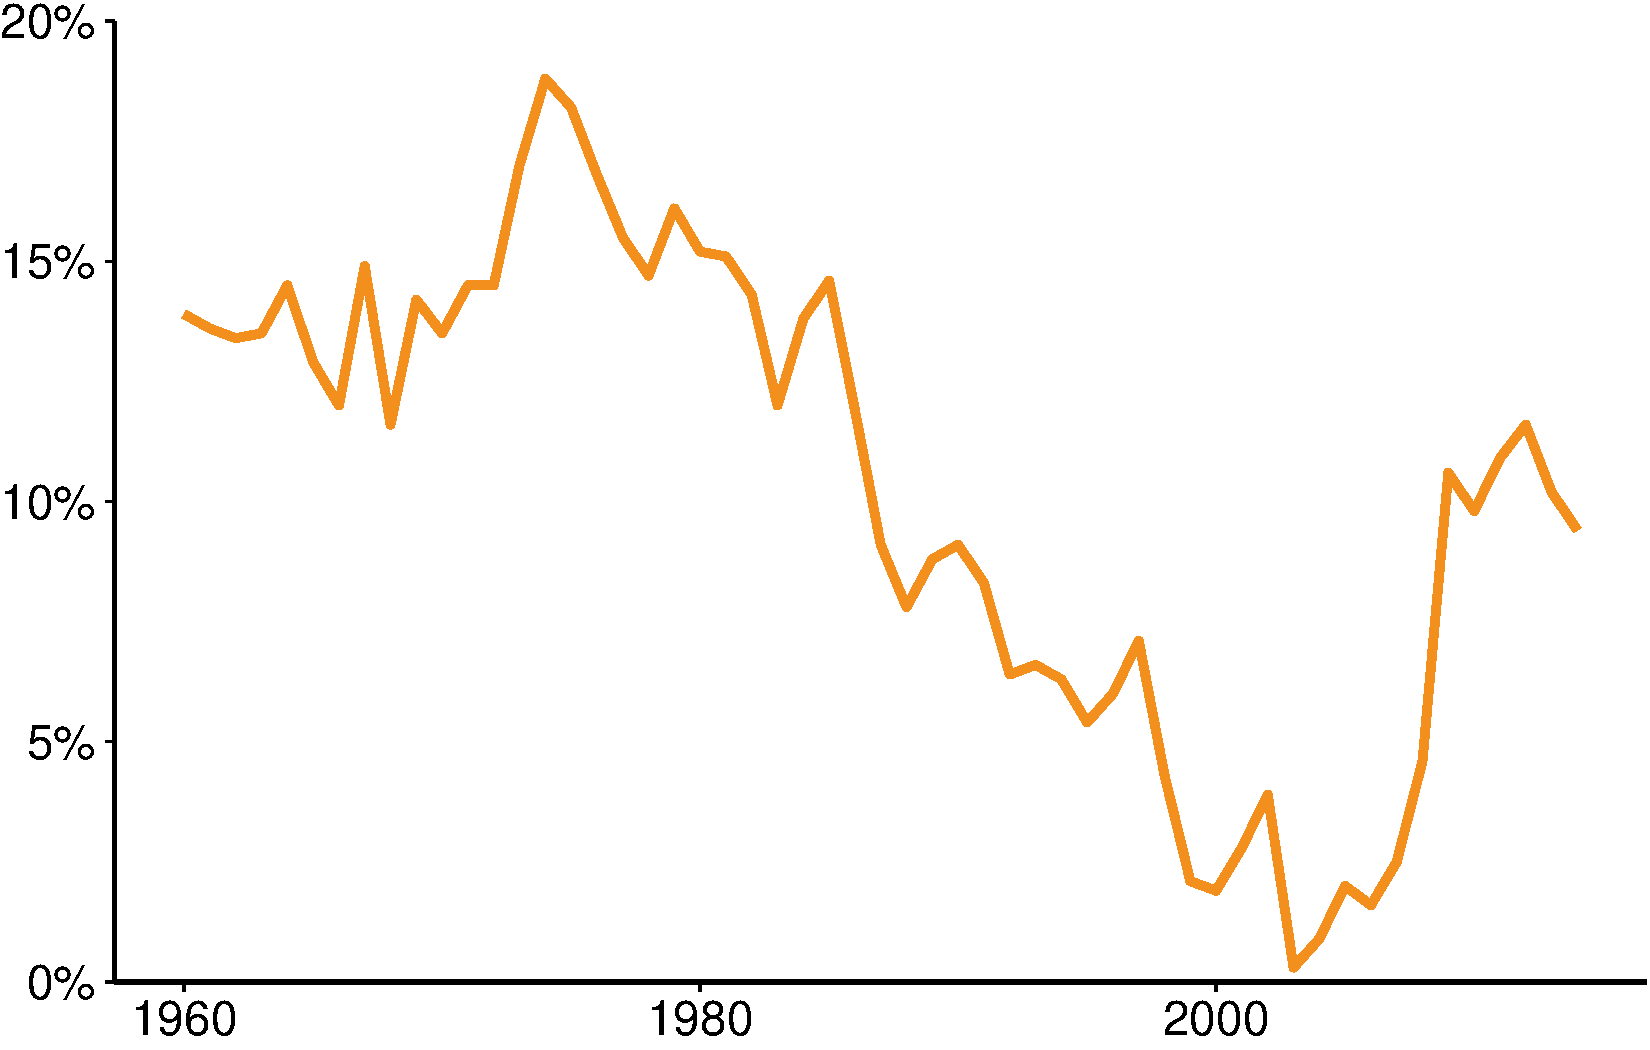
\includegraphics[width=\columnwidth]{atlas/Households_are_saving_more-1.pdf}
\notes{Household saving calculated as a residual item by deducting household final consumption expenditure from net household disposable income. Net disposable income is calculated by deducting depreciation from gross disposable income. See: \textcite{ABS2007}.}
\end{minipage}
\hfill 
\begin{minipage}[t]{\columnwidth}
\captionwithunits{\dots\ and\label{fig:GST-2} spending less on GST-liable goods and services}%
{Spending by category, 1999 = 100}
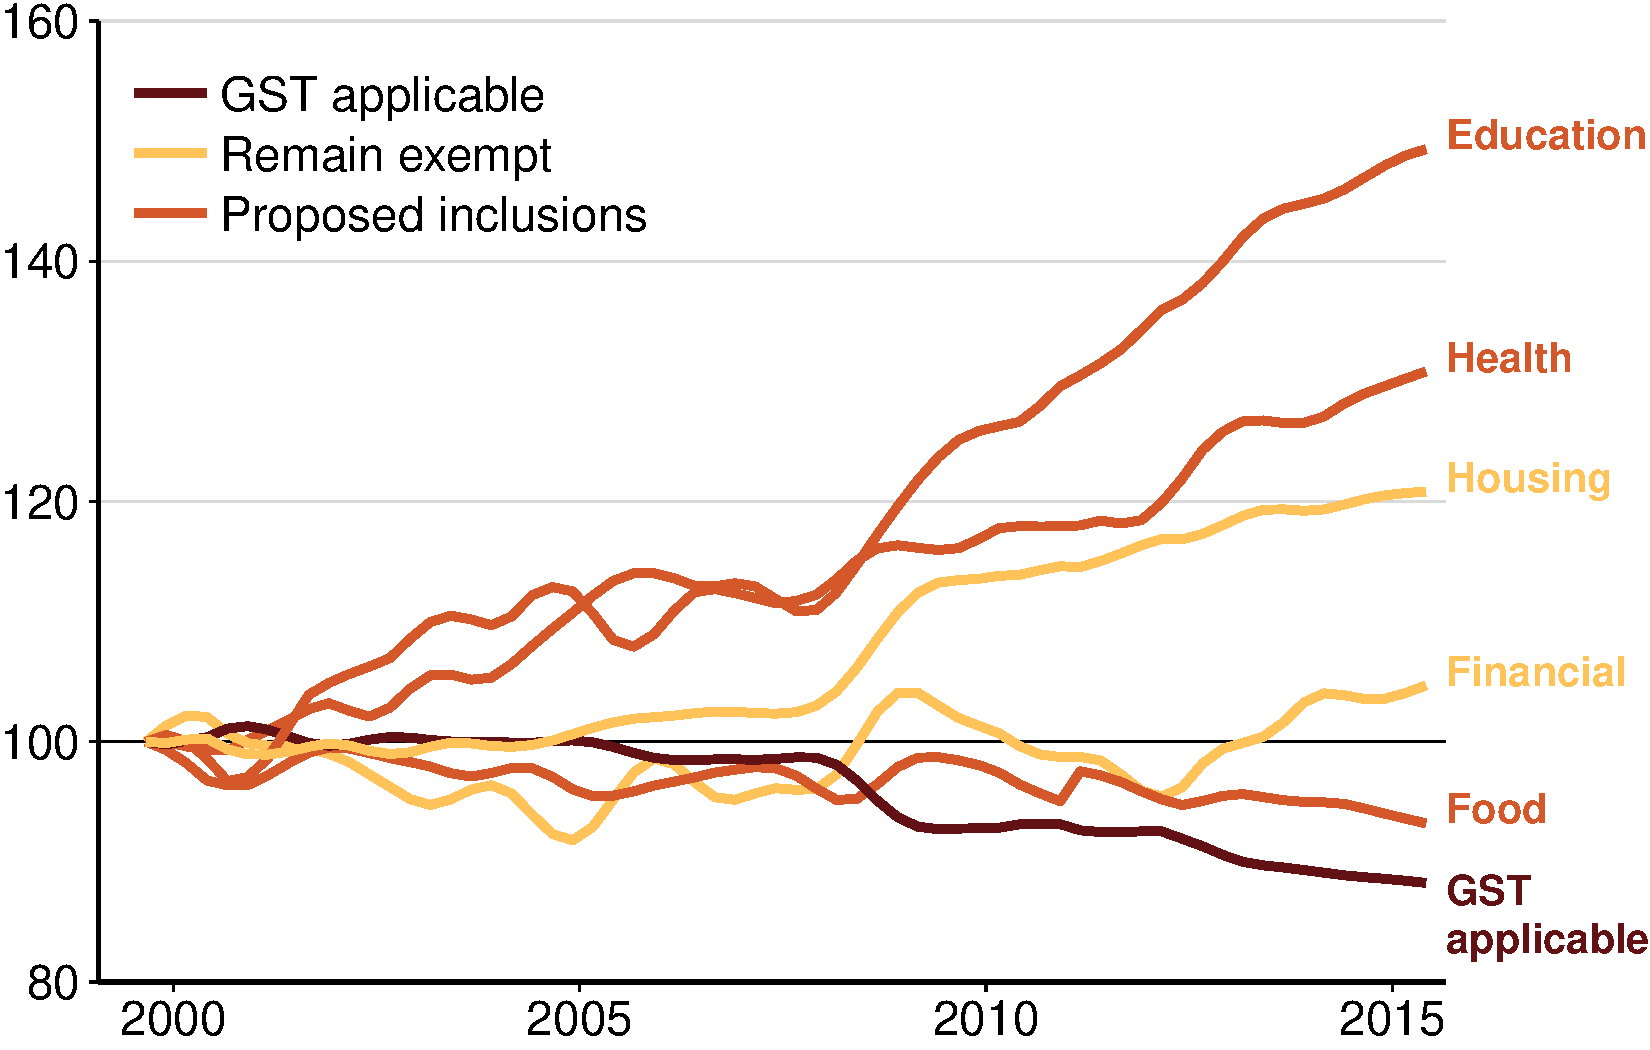
\includegraphics[width=\columnwidth]{atlas/Spending_less_on_GST_liable-1.pdf}
\notes{Some food and financial services are subject to GST but because we cannot identify them separately in the National Accounts we have classified these categories as GST exempt for this analysis.}
\end{minipage}


\source{\textcite{ABS2015-NationalAccounts-ExpenditureProduct}; Grattan analysis.}
\end{figure*}

Not only are Australia’s revenues from broad-based consumption taxes low by international standards, they are shrinking relative to the economy. In the decade to 2014-15, GST revenues fell from almost 4.0 to 3.4 per cent of GDP.  Households saved more of their incomes (\Vref{fig:GST-1}) and what they spent increasingly went on GST-exempt items, particularly housing (\Vref{fig:GST-2}).\footnote{See \textcites{Treasury2014-Budget-Papers-2014-15}[][38--41]{PBO2014TrendsAustralianGovtReceipts1982to2013} 41 for a more detailed discussion of these trends.} 

There is no obvious reason for these trends to reverse in the foreseeable future. Savings rates are now closer to long-run averages, with low savings rates in the early 1990s and 2000s looking like a historical anomaly.\footnote{The decline in the household savings ratio coincided with a period in which household wealth and debt levels grew strongly (\textcite[][38]{PBO2014TrendsAustralianGovtReceipts1982to2013}).}  The proportion of household incomes spent on health is forecast to grow.\footcite[][28]{DaleyWoodWeidmannEtAl2014}  And the share of incomes spent on housing may also continue to increase: land supply is finite, and new housing supply is struggling to meet the demands of a growing population.\footnote{Ultimately future housing prices will depend on population growth, household size and whether supply of new properties keeps pace with the growth in demand. See: \textcite[][7]{RBA2014SubmissionAffordableHousingInquiry}.}

The GST has not been – and without reform may never be – the ‘growth’ tax the states were originally promised. \footcite{CostelloBudgetSpeech2000-01}

\section{Consumption taxes harm the economy less than many other taxes}\label{sec:GST-1-2}
Broad-based consumption taxes such as the GST are relatively efficient taxes. They drag less on economic efficiency than many state government taxes including payroll taxes\footnote{In theory, broad-based payroll taxes and consumption taxes are equivalent, but the range of exceptions and thresholds provided by state governments for payroll taxes have considerably reduced their efficiency.}  and stamp duties.\FOOTNOTE{See \Vref{box:PROP-1}.}  

Consumption taxes are efficient for many reasons. They are relatively difficult to avoid\footcite[][274]{HenryTaxReview2010}  and create fewer distortions in decisions to work, save and invest. 

A consumption tax treats current and future consumption equivalently, so it creates no distortion in savings decisions. By contrast, income taxes somewhat deter savings by taxing the returns on those savings.  Generating more revenue from taxes on consumption should reduce this distortion. But the economic payoff may not be large: tax rates make relatively little difference to savings decisions of high-income earners who do most of the saving.\footnote{Under an income tax system, individuals pay tax on their labour income (regardless of how much they save) and then again on any returns to saving that income. See: \textcite{HenryTaxReview2010}} \DEVIATION{Not possible to decipher}   

An increase in consumption tax also acts as a lump sum tax on accumulated wealth, and so collects more from households such as retirees that are living off savings. The economic drag from these increased tax collections is low. Such households otherwise contribute far less to tax collections than do working households on equivalent incomes.\FOOTNOTE{See \Vref{chapter:FISCAL-3}.}  And their contribution relative to younger households is falling as a result of superannuation tax breaks. Our Wealth of Generations report showed that households over 55 are reducing their share of tax paid, despite increasing wealth relative to younger households.\footcite[][27]{DaleyWoodWeidmannEtAl2014}  Low income older households will receive additional welfare as compensation for price increases through our proposed compensation package (\Cref{chapter:GST-3}).

Income taxes affect the incentives to work more than consumption taxes. Both taxes reduce the amount that can be purchased from an hour of work. In theory a labour income tax and an equivalent consumption tax have an identical effect on work incentives.\footnote{For a summary, see: \textcite[][458]{McCaffry2008}.}  But in practice, consumption taxes may discourage working less than income taxes because their impact on spending power is less obvious. Consumption taxes are less salient: there is some experimental economics evidence that people notice lower nominal wages (due to income tax) more than lower real wages (due to a consumption tax).\footnote{\textcites{BlumkinRuffleGanun2012}{SausgruberTyran2005}. This is because of the ‘money illusion’: individuals tend to think in nominal rather than real terms.}  Treasury estimates that a broad-based consumption tax causes a somewhat smaller economic drag than a flat rate labour income tax.\footnote{Treasury estimates that the ‘marginal excess burden’ – the loss of economic activity for each dollar of tax levied – is 21\,c for a flat labour income tax and 17\,c for a broad-based GST. See: \textcite[][25]{Treasury2015ReThink}.}  

Further, the combination of income tax scales and the withdrawal of means-tested welfare benefits can discourage working because they result in low rates of take home pay. The disincentives are larger for low-income workers and those working part time (\Cref{sec:GST-3-4}).\footnote{\textcites{ProductivityCommission2015-Tax-and-transfer-incidence}{HardingNguVuPayneEtAl2009}{Reference-Group-On-Welfare-Reform-to-the-Minister-for-Social-Services-2015}, 
which recommended mechanisms to improve these incentives. \textcite{Apps2015} argues that GST could exacerbate this problem because the unit of taxation is the household – \ie, all household consumption is taxed at a flat rate. In contrast, the progressive nature of labour income allows a lower tax rate for the second earner on the lower wage. Our proposed compensation package that targets income tax cuts at the low and middle brackets (\Cref{chapter:GST-3}) will help mitigate this concern.}  Higher income tax rates as a result of bracket creep can materially reduce workforce participation of middle-income earners.\FOOTNOTE{See \Vref{fig:FISCAL-4}.}  

Overall, higher consumption taxes should hurt the incentives to work, save and invest less than higher income taxes. Incentives to work can be improved if income tax cuts introduced with the GST are targeted at low and middle brackets (\Cref{sec:GST-3-4}). And potential disincentives to work as a result of higher welfare benefits to compensate poorer households for a higher GST can be managed if the compensation package is carefully designed. (\Cref{sec:GST-3-3}). 

\chapter{A broader base or higher rate?}\label{chapter:GST-2}
GST revenue collections can be increased either by broadening the range of items that are subject to the tax (‘broadening the base’) or by increasing the rate above the current 10 per cent. Economists generally favour broadening the base because it is simpler and more efficient. But increasing the rate could be a satisfactory ‘second best’ if it is too politically difficult to broaden the base. A brave government might do both. 

\section{The GST could be broadened}\label{sec:GST-2-1}
Australia’s GST covers 47 per cent of the potential consumption base. This is well below the OECD average of 55 per cent (\Cref{sec:GST-1-1}).

Several expenditure categories are currently excluded from the GST.\footnote{The OECD draws a distinction between goods and services taxed at reduced rates, including a zero rate, and goods that are exempt (input-taxed). Under this classification, in Australia, health, education, fresh food, water and childcare are taxed at a reduced (zero) rate and financial services and housing are exempt.}  Broadening the base to include fresh food, education, health, childcare, water and sewerage could raise over \textbf{\$17~billion} (\Vref{fig:GST-3}), based on household spending levels in 2014-15. Revenues would increase over time, as household spending on these goods and services grows.\footnote{All costings in this paper are for 2014-15. Using historical data allows more robust modelling of the distributional impacts of changes in the GST and proposed compensation packages. As GST revenues are forecast to grow, the revenues to government from increasing or broadening the GST will be higher in future years.} This figure takes into account the effects of changes in consumer behaviour due to the increased prices in these categories. 

\begin{figure}
\captionwithunits{Including fresh food, health,\label{fig:GST-3} education, and other categories in the GST could raise over \$20~billion}%
{Potential GST revenue of excluded items, 2014-15}
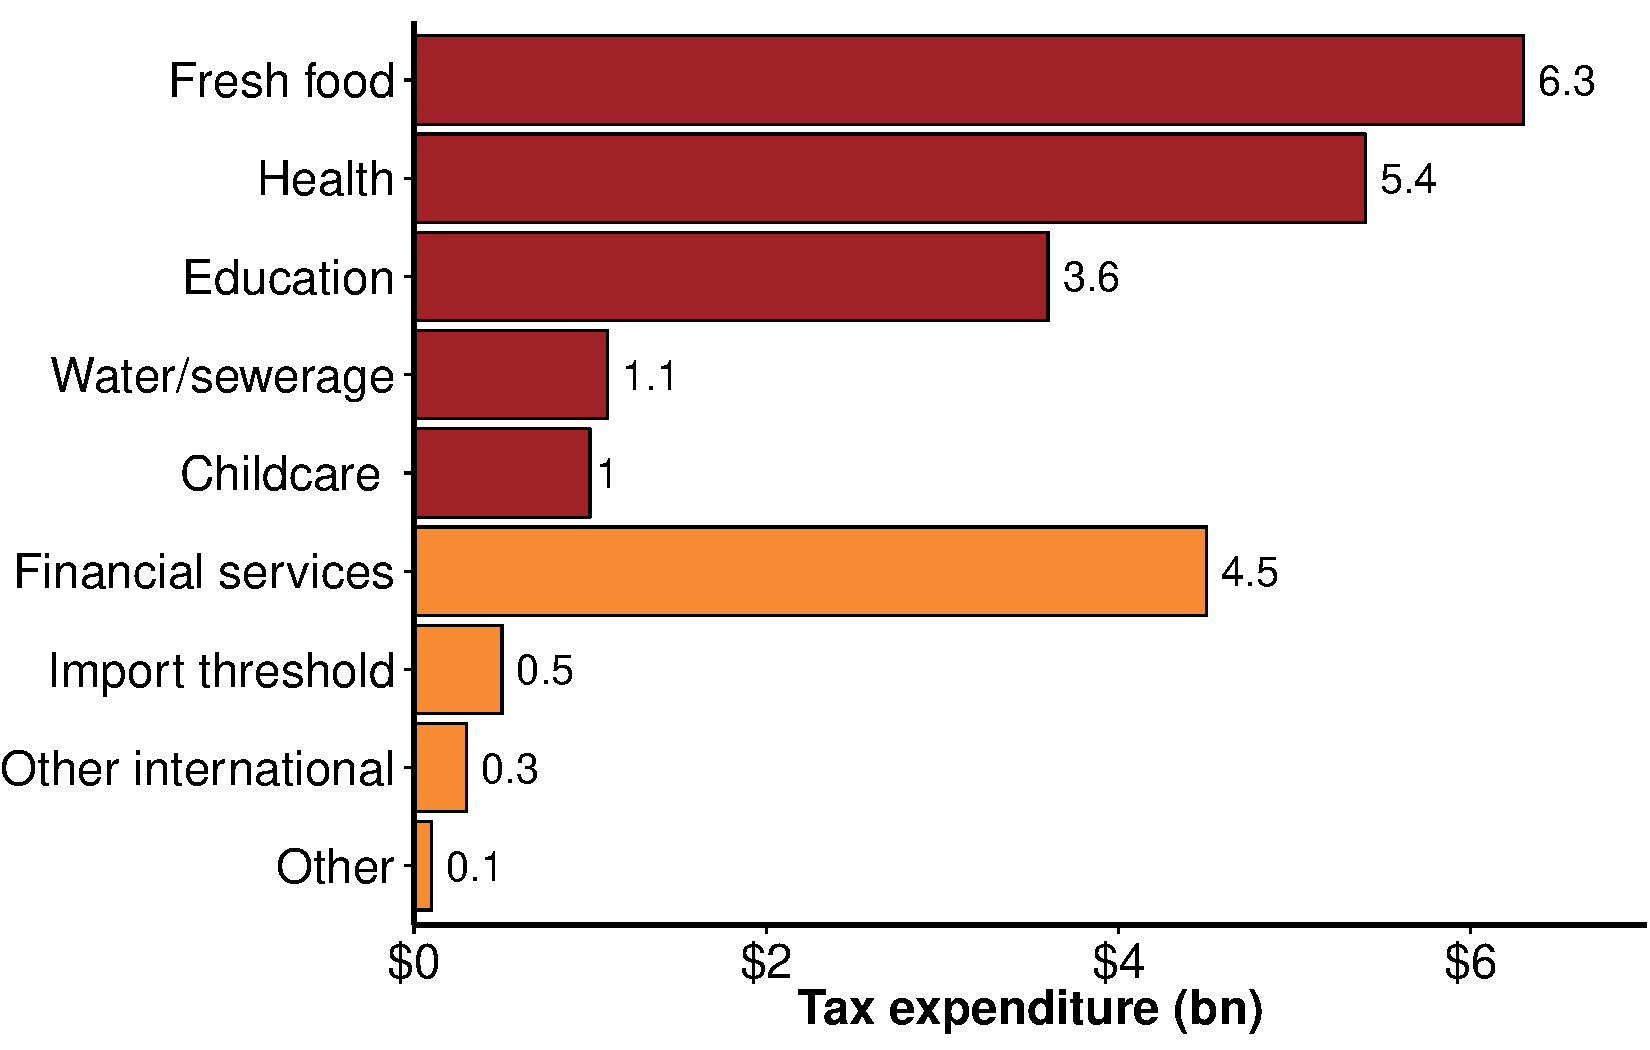
\includegraphics[width=\columnwidth]{atlas/GST_revenue_of_excluded_items1415-1.pdf}
\notes{Excludes housing services as a comparable estimate is not available.}

\source{\textcite{Treasury2015TES2014}; Grattan analysis.}
\end{figure}

This would leave exemptions in place for financial services, existing residential housing, and some other smaller spending categories.  These are currently ‘input taxed’. Financial service providers pay GST on their inputs but do not charge GST to customers.  As a result, households are under-taxed because there is no tax on the value-added component of financial services, and businesses are over-taxed because they cannot claim GST offsets for the taxes on the inputs for these services.\footnote{Financial services exemptions include supplies by charitable organisations and administrative exemptions for very small businesses. See \textcite[][169]{Treasury2014TES2013}.}

Similarly, home owners pay GST on the costs of maintaining and upgrading their house, but there is no GST levied on the ‘imputed rents’. In order to maintain neutrality between owner-occupiers and investors, GST is not applied to rents for investment properties.

Ideally these services would be taxed in the same way as other consumption.\footcites{Freebairn2013}[][52]{HenryTaxReview2010}  But taxing the full value added of these services is complex. It is not easy to determine the appropriate margin on which to calculate the tax.\footnote{The invoice basis on which GST is determined for most other goods and services is very difficult in circumstances where there is an implicit fee or margin arising from financial transactions entered into over a period of time with a number of customers. See: \textcites{Evans2015}{Davis2015} for more discussion.}  
Consequently, these categories are excluded from value added tax in almost all OECD countries.\footnote{\textcite[][21]{OECD2014}. The Treasury potential revenue gain estimates in \Vref{fig:GST-3} assume away this difficulty.}  

For \textbf{financial services}, the South Australian Government has proposed a ‘financial institutions duty’ which is broadly equivalent to the GST but easier to implement.\footcites{Evans2015}{Weatherill2015}  The duty is a supplementary tax on the margins between the rates charged by financial institutions and the rates at which they borrow. There remains some administrative complexity – for example, determining the best way to exclude business banking\footcite{Davis2015}  – but such a duty is worth considering as a way to tax the ‘value added’ from financial services. 

The Australian Government has already announced proposed changes to the \textbf{GST treatment of imports} from 1~July~2017. Imports worth less than \$1000 are currently exempt from the GST. Under the new policies, GST will apply to all imported digital goods and services and physical goods.\footnote{In other words, the value threshold will be set at zero. The measure to include GST on cross-border supplies of digital goods and services was included in the May 2015 Budget,
\textcite[][20]{Treasury2015BudgetPapers201516}. The government announced a policy to charge GST on cross-border supplies of physical goods under \$1000 following agreement with the state and territory treasurers at a meeting in August 2015. \textcite{Hockey2015--GST-import-threshold}.}  The requirement to collect and remit GST will be imposed on the overseas vendor. Only vendors with an Australian turnover of \$75,000 will need to register for and charge the GST.

The policy imposes a fixed cost on overseas retailers selling to Australians, as they would need to implement systems that apply specifically to any purchaser based in Australia. This impost would be relatively small for retailers that sell large volumes to Australians, like Amazon and Netflix. Some of these have already suggested they will register for the GST.\footnote{Netflix indicated they will continue to comply with local tax obligations. Apple already charges GST on its digital downloads in Australia. See: \textcite{Coorey2015-Netflix}.}  However, it is not clear what legal recourse will be available to the government if overseas vendors do not choose to register.%
\footnote{The Low-Value Parcel Processing Taskforce that explored this issue in 2012 said that GST obligations imposed directly on international suppliers would ‘likely be non-enforceable, and hence rely on voluntary cooperation by suppliers’. \textcite[][139]{Treasury2012c}}  The former Treasurer Joe Hockey argued that ‘global pressure’ would force retailers to comply.\footcite{Hockey2015--GST-import-threshold}  

\section{Increasing the GST rate}\label{sec:GST-2-2}
An alternative to broadening the base of the GST is to increase the rate. Australia’s 10 per cent rate is low by international standards. It is the fourth lowest value-added tax rate in the OECD, and considerably below the OECD average of 19 per cent.\footcite{OECDKoreaInstitutePublicFinance2014-Distributional-Effects-Consumption-Taxes}  

Increasing the rate of the tax from \textbf{10 to 15~per~cent} could raise as much as \textbf{\$27~billion}, based on GST collections in 2014-15. This does not factor in behavioural change, although it is unlikely that much revenue will be lost from people shifting their spending towards GST free goods and services.\footcite{KPMGEconotech2011-GST}  As discussed in \Cref{box:GST-1}, consumption of GST exempt categories (particularly fresh food, health and education) is not affected much by their price relative to other goods and services.

\begin{bigboxC*}{Change in consumer choices due to a broader GST}{box:GST-1}
Broadening the GST will increase the relative price of fresh food and private health and education services. But empirical evidence suggests that behaviour won’t change much as a result. 

Treasury finds that demand in the \textbf{fresh food} category is inelastic – that is, a price rise will not lead to much change in consumption. It estimates that a 10 per cent increase in tax on food would only reduce consumption by 1.6 per cent (\textcite{Treasury2015TES2014}).

A study for the Rural Industries Research and Development Corporation using data from the ABS Household Expenditure Survey also concluded that demand for fresh foods such as milk, bread and fresh vegetables does not change much if relative prices change. The estimates suggest that a 10 per cent increase in price would reduce consumption by between 2 and 7 per cent for these categories. For fresh fruit and other dairy, consumption is estimated to fall 10 per cent if prices rise by 10 per cent. Purchases of various types of meat (beef, lamb, pork, chicken) are estimated to respond even more to changes in price (\textcite{UlubasogluMallickWadudEtAl2015}). 

However, these estimates only capture changes in demand if prices change for only one type of food, such as pork. Many of the people no longer buying pork will switch to buy more of other types of meat, or other fresh food. It is likely that people will reduce their overall consumption of fresh food by less than these category estimates if fresh food prices increase across the board. 

Studies of private health insurance in Australia and internationally have found that consumers are not very responsive to price changes. Estimates of the price elasticity of supplementary private health insurance (insurance that provides more choice or faster access relative to universal health care) range from between 0.2 and $-$0.5, suggesting that demand would fall less than 5 per cent in response to a 10 per cent GST (\textcite{Cheng2013-health-insurance-elasticity}). 

Demand for hospital insurance is likely to change even less with a GST. Policies such as lifetime health cover loading, and the Medicare levy surcharge, provide strong incentives for those aged over 30 or on higher incomes to maintain private cover unless prices increase dramatically (\textcite{ATO2015-Private-Health-Insurance-rebate-Medicare-levy-surcharge}). 
Consequently, Treasury estimates that demand for private \textbf{medical and health services} may only fall by 1.4 per cent in response to a 10 per cent GST. 

However, governments may face pressure to reduce co-payments for some health services if price increases disproportionately affect disadvantaged groups. This would somewhat offset potential revenue gains from applying the GST to these services. 

Treasury’s elasticity estimate for \textbf{private education services} suggests that a 10 per cent tax on education will lead to a 10 per cent decrease in demand. But this includes the effects of reductions in demand for discretionary courses for which students are less likely to switch to public providers. Price changes are likely to have much less impact on schooling choices. Historical trends in Australian \textbf{private school enrolments} suggest that parents are not particularly price sensitive. Between 1990 and 2007, average fees roughly doubled in real terms for both Catholic and Independent schools. During this period their enrolment share \emph{increased} by around two and five percentage points respectively (\textcite{NousGroup2011-Funding-for-Schooling}). 


\end{bigboxC*}


\section{Broadening the GST will make it simpler, more efficient, and more durable}\label{sec:GST-2-3}
A broader base for consumption taxes minimise distortions in decision making. When purchases of all goods and services are taxed at the same rate, people consume the goods and services they value most, given their price. When differential tax rates apply then there are welfare losses: people are induced to consume relatively more of the lower taxed goods and less of the higher taxed goods than they would otherwise prefer.\footcite{AtkinsonStiglitz1976}  This is particularly true when different tax treatment is applied to goods or services that are substitutes. For example, remedial massage attracts GST while both osteopathy and chiropractic services are GST free.\footcite[][\S38-7]{GST-Act-1999}  Broadening the GST would remove these distortions.  

There are other reasons to favour a broad-based tax. Exemptions create administrative costs for businesses that deal with both exempt and non-exempt goods, and compliance and enforcement costs for tax administration agencies.\footnote{Currently private schools and hospitals are classed as charities (see \textcite{ACNC2015}) so there would need to be some amendments to the charities exemption to apply the GST to these services.}  And grey lines create opportunities for tax avoidance and lobbying to exclude particular goods.\footcite{Freebairn2015}  While arguably most of these costs have already been sunk, new fronts in the debate open up from time-to-time.\footnote{For example, the recent proposal to remove GST from feminine hygiene products. However, the proposal failed because it did not receive unanimous support from State and Territory governments. See: \textcite{Hockey2015-Federal-Finance-Relations}.}  

In a recent national poll, a majority of senior Australian economists favoured broadening the base of the GST rather than increasing the rate.\footnote{Recent poll of the 49 senior economists on the National Economic Panel, \textcite{NationalEconomicSocietyAustralia2015-GST}.}  Most thought it would increase efficiency and simplicity. By contrast, the one third who disagreed (the balance were undecided) were either sceptical about the net efficiency gains or had doubts that compensation would be adequate to address the effects of a more comprehensive GST for those on low incomes.

Including spending on education and health in the GST will also help address the problem of ‘base erosion’. Spending on health in particular is expected to rise faster than income (\Cref{sec:GST-1-1}). Including health and education in the GST base will ensure revenues from the tax better keep pace with economic growth, as well as aligning more closely with state government expenditures. 

On the other hand, a 15 per cent GST would raise more money than broadening the base. This is attractive given the need for Commonwealth and state governments to address their revenue shortfalls in the most efficient way. If higher revenues are a priority, then a simultaneous rate increase to 12.5 per cent and base broadening – which would raise about \$35~billion a year – would be the most efficient way to achieve them. 

\section{Social purposes of existing exemptions could be served better by other means\label{sec:GST-2-4}}
Some defend the existing exemptions because they send consumers worthwhile price signals to consume more healthy fresh food and to spend more on private health and education in ways that reduce the pressures on the public systems. 

However, GST exemptions are an inefficient way to pursue these ends. There are any number of goods and services the government might want to promote or deter. But broad tax exemptions are a blunt instrument for fine-tuning consumption habits. There are few items with market failures so large that they justify governments imposing differential tax treatment despite the efficiency costs.\footcite[][163]{MirrleesAdamBesleyEtAl2011}  For these items, government can design ‘sin taxes’ specifically aimed at the problems.\footnote{In these examples the purpose of the taxes is to change relative prices and therefore behaviour rather than to simply raise money. \textcites{MirrleesAdamBesleyEtAl2011}{HenryTaxReview2010}.}  For example, if governments want to use taxes to encourage better diet, then a high tax rate targeted at foods high in sugar and salt would be much more effective than a relatively small shift in the price of all processed food.\footnote{For example, the Australian Government’s Preventative Health Taskforce recommended a review to consider increasing taxes on energy dense foods. \textcite[][15]{Preventative-Taskforce2008-Australia-Healthiest-Country-by-2020}.}  In any case, empirical evidence indicates that there would be relatively little change in consumer behaviour if government broadened the GST to include fresh food (\Cref{box:GST-1}).

Others argue that a GST on private health and education services will give public providers an advantage over private providers. But governments don’t aim for a level playing field in health and education: they explicitly provide higher subsidies for those using the public systems. 

A more serious objection is that charging GST on private health and education could reduce total government revenue if it led people to switch from less subsidised private services to more subsidised government services. But the evidence suggests that switching would be limited (\Cref{box:GST-1}). And in any case, there is now evidence that the government subsidy provided to public schools is not much greater than the subsidy for private schools once the relative disadvantage of the student base is taken into account.% 
\footnote{A recent study using MySchool data to adjust for relative disadvantage suggests that Catholic private schools receive only slightly less (and in some cases more) government funding per student for a given range of student disadvantage. Other independent schools receive somewhat less but the gap is decreasing over time. \textcite{BonnerSheperd2015}.}

\chapter{A targeted compensation package}\label{chapter:GST-3}
Opposition to increasing Australia’s GST is often motivated by concerns about how low-income households would be affected. If governments want to ensure that disadvantaged households are not left significantly out of pocket, compensation will be required. A compensation package should also maintain incentives for workforce participation, particularly for low- and middle-income earners, who are most responsive to changes in effective tax rates. This means a combination of tax cuts and higher welfare payments.  

But any GST reform package aiming to provide revenue to state governments to fund growing health and education spending,\FOOTNOTE{The decision in the 2014-15 Commonwealth budget to withdraw from the National Health Reform Agreement and to no longer fund growth in real per person hospital spending precipitated the current public discussion about increasing the GST. See: \Vref{sec:FISCAL-4-3}.}  or to reduce government deficits, must be revenue positive. Some people will need to pay higher net taxes. Even if the package is budget-neutral, the political need to over-compensate low-income households in order to protect the most disadvantaged will lead to some other households paying more tax in total.

This will be difficult for governments that have become accustomed to ‘buying’ tax reform. The GST and the introduction of the carbon tax were both accompanied by a package of generous tax cuts and increases to welfare benefits that left very few households worse off (\Vref{box:GST-2}). A history of yielding to demands that there be ‘no losers’ has changed the political economy of reform. Politicians have arguably become less adept at prosecuting the case for difficult changes.\footcite[][80]{Megalogenis2010}  And the public have come to expect that medicine will always arrive with a spoonful of sugar.\footcites[][45]{Megalogenis2010}{Henry2015}   But without revenue-positive reforms, the budget pressures we outlined in \Cref{part:FISCAL} will only continue to increase.  

The other challenge for the federal government is reconciling GST reform with its claim that it will not increase the tax burden.\footnote{See, for example, \textcite{Morrison2015-QnA-Melbourne-Institute}.}  Even budget-neutral GST reform will increase taxes as a share of the economy because some money will be spent on compensating people on welfare. To stop the tax burden increasing, all the GST revenue would have to be given back as income tax cuts. Any associated increase in welfare payments would then \emph{increase} the deficit – unlikely to be tenable in a period when the government is trying to do the opposite. 

Our proposed package balances the need for fiscal consolidation with fairness and efficiency. It overcompensates the bottom 20 per cent of the income distribution on average, mainly through higher welfare payments. In terms of their real purchasing power, most of the poorest Australians would be no worse off, and the majority would be better off. Modest tax cuts focused on the low and middle thresholds would maintain or improve the incentives for work participation and ensure that most low- and middle-income earners are also better off. Around 40 per cent of the additional revenue would be left over. The potential uses for this money are discussed in \Cref{chapter:GST-4}. 

\begin{bigboxC*}{Buying reform -- the GST and carbon price compensation packages}{box:GST-2}
The introduction of the GST in 2000 was accompanied by cuts to personal income tax and increases in welfare benefits.

Personal income tax changes costing around \textbf{\$13 billion} a year included: an increase in the tax-free threshold; a reduction in tax rates at the lower end; and an increase in the threshold for the top marginal tax rate. 

The objective of this consumption tax / income tax ‘swap’ was to improve the efficiency of the tax system by improving incentives for work.

Pensions and other social security payments were also increased by 4~per~cent across the board to compensate welfare recipients for higher prices following the introduction of the GST. These increases cost around \textbf{\$2 billion} in 2002-03. 

Family payments were increased even more, at a cost of around \textbf{\$2.5 billion} a year. These increases were designed to compensate for the higher cost of living following the introduction of the GST and to provide greater recognition of the costs of raising a family. 

In 2002-03, the GST raised around \textbf{\$30 billion while other taxes worth \$25 billion} – wholesale sales tax and state indirect taxes – were abolished (or proposed to be abolished) as part of its introduction. Overall, the package \textbf{overcompensated households} by about \textbf{\$12~billion} a~year.

While the package was sold on the basis that everyone would be better off, the structure of the tax cuts meant the middle class benefited in particular. Overall, the package increased inequality. \textcite{Saunders2004} shows that incomes at the 90th percentile increased markedly relative to the 10th percentile in the year following the introduction of the GST.

In contrast, the Household Assistance package for the \textbf{carbon price} pushed money towards those at the bottom of the income distribution. 

Around half the \textbf{\$4 billion} revenue from the first year of the carbon tax was given to households as compensation.  

The compensation package included higher family payments and pensions, and tax cuts to all taxpayers earning up to \$80,000. The assistance package actively targeted households at the lower end of the income distribution, with the goal of fully offsetting the cost of living increases for \textbf{low-income households} and helping to meet the increases in costs for \textbf{middle-income households}. 

Around 90 per cent of households received some compensation. There was also a fund to ease transition costs for business and community sector organisations. Overall the package over-compensated households for the increases in living costs: the average assistance of \$10.10 per week was higher than the average cost increases of \$9.90. 

\boxsources{\textcites{Costello1998}{Treasury2002}{Eccleston2006}{Treasury2011-Supporting-Aust-Households}{Treasury2012}{ParliamentaryLibrary2011}.}

\end{bigboxC*}

\section{GST has slightly more impact on low-income households}\label{sec:GST-3-1}
Many claim that the GST should not be increased because it would be unfair to low-income households.\footnote{For example, Labor Minister Tony Burke cited in \textcite{Hutchens2015-ALP-not-support-GST}.}  The argument is that governments should seek to protect the welfare of the bottom 20 per cent of taxpayers because they are obliged to protect the welfare of the most vulnerable.\footnote{See \textcite[][21]{Daley2013} for further discussion.}

The fairness of the GST can be judged in different ways. 

In \emph{absolute amounts}, a GST collects far more from high-income households:\footcites{OECDKoreaInstitutePublicFinance2014-Distributional-Effects-Consumption-Taxes}{Freebairn2013}{HenryTaxReview2010}
the exemption for fresh food, for example, saves the richest 20 per cent of households around \$1000 per year, compared to an average of \$420 per year for the poorest 20 per cent of households.\footnote{Grattan estimates based on \textcites{Treasury2015TES2014}{ABS2011HES0910curf}.}

However, the fairness of a reform is often judged by looking at the \emph{percentage} of a person’s resources affected.  

Poorer households pay substantially more GST \emph{as a proportion of their income} because they spend more of their incomes than richer households. Savings rates increase with incomes.\footnote{The bottom quintile of households by income spend around 40 per cent more than they earn before taxes and transfers, while the top quintile saves the equivalent of 20 per cent of their gross income. 

At first glance, analysis by the Productivity Commission (PC) casts doubt that the GST is regressive  – it shows that poorer households pay only slightly more GST as a proportion of their income that richer households. However, this is because the PC presents GST burden as a share of disposable income but ranks households based on income levels before tax and transfers. See: \textcite[][74--76]{ProductivityCommission2015-Tax-and-transfer-incidence}.  Using the same measure of income to assess the GST burden and rank household incomes – either both gross or both disposable – we find that poorer households pay substantially more GST as a proportion of income.
} 

But a GST is less regressive when the tax burden is considered as a \emph{percentage of consumption}. It is arguable that this is a better measure of the fairness of a consumption tax. Most households that are low-income at a point in time – students, retirees, or the short-term unemployed – have much higher lifetime incomes. These people smooth their consumption by borrowing or drawing down on their savings when their income is low. At these times they pay more consumption tax as a share of income. They pay a lower share when their earnings are higher. Consequently, the proportion of current consumption paid in tax can give a better indication of the tax burden on a household over their lifetime.\footnote{\textcites[][275]{HenryTaxReview2010}[][34--36]{OECDKoreaInstitutePublicFinance2014-Distributional-Effects-Consumption-Taxes} If a household saves in net terms over their lifetime (\ie, they pass on some assets) then some of the tax burden will be deferred until the money is spent by the next generation.}

All households pay a similar amount of GST as a proportion of their consumption.\footcite[][41]{OECDKoreaInstitutePublicFinance2014-Distributional-Effects-Consumption-Taxes} Broadening the GST to include fresh food, and private spending on health and education would lead to a bigger increase in GST as a share of consumption for lower income households. Lower income households spend a little more on fresh food and health as a proportion of spending, which are currently exempt from GST. This outweighs their lower relative spending on education and childcare, the other major categories of expenditure currently exempt from GST, as shown in \Vref{fig:GST-4}.

\begin{figure}
\captionwithunits{Poorer households devote a little more of their spending to goods and services included a broader GST\label{fig:GST-4}}%
{Percentage of spending by gross household income quintile, 2009-10}
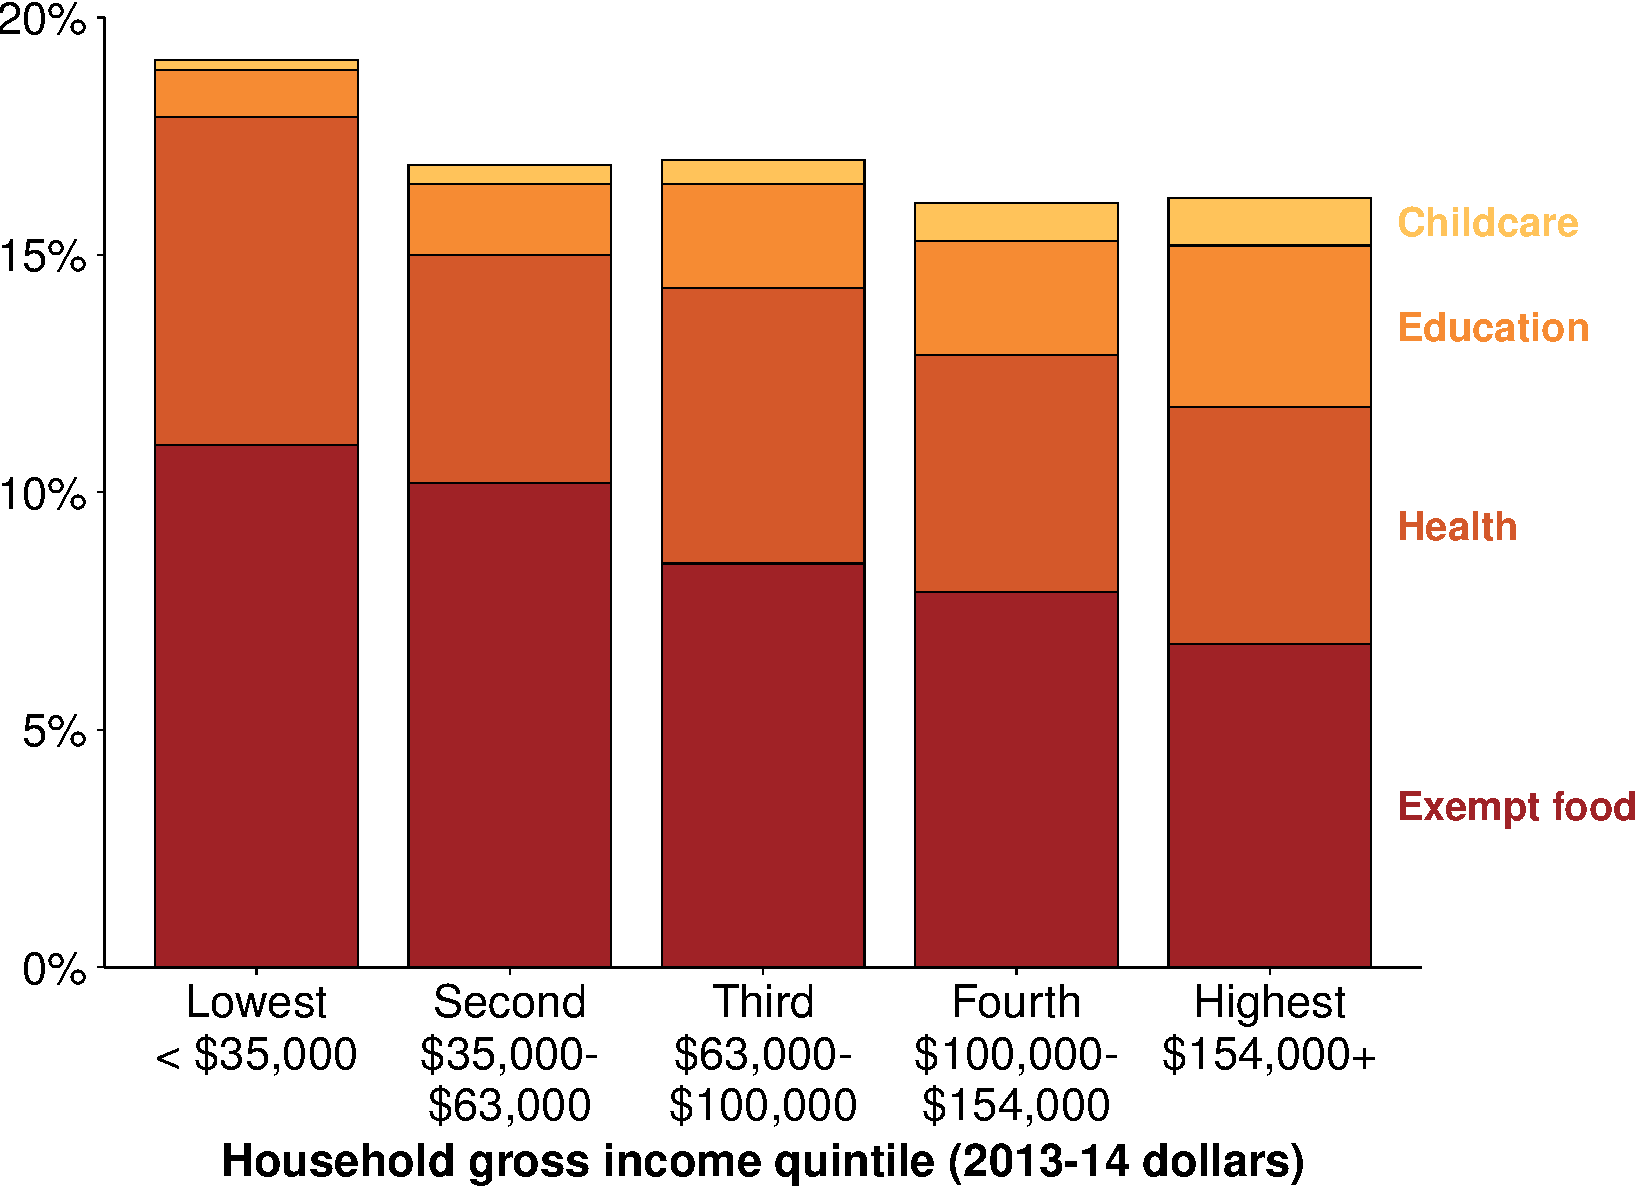
\includegraphics[width=\columnwidth]{atlas/figure/GST-Figure-4-1-tikzd.pdf}
\source{\textcite{ABS2013t}; Grattan analysis.}
\end{figure}

Overall, the differences are small: if the GST were broadened and purchasing patterns are unchanged, poorer households would pay on average an extra \$19 per \$1000 spent, compared to \$16 per \$1000 spent for the top 20 per cent of households. 

If the GST rate were raised but not broadened, high-income households pay slightly more:  \$26 per \$1000 spent compared to \$25 per \$1000 spent by poorer households. Of course, these averages conceal substantial variation in spending patterns between people in a given income group (\Cref{sec:GST-3-2}).

While some argue that a tax can be fair providing it doesn’t disproportionately impact poorer households, many are concerned by tax reforms that would take \emph{any} resources from the most vulnerable. To ensure the fairness of our GST reform proposal, we structure a compensation package so that \textbf{on average the poorest 20 per cent of households are at least fully compensated for the higher tax.} 

Fairness – and political pragmatism – also supports some compensation for middle income households. Our package ensures that most \textbf{households earning up to \$100,000 are compensated for at least 75 per cent of the cost of the higher GST.}

Introducing changes to the GST as part of a broader tax reform package which includes more progressive measures – such as better targeting of superannuation tax concessions\FOOTNOTE{See \Cref{part:SUPER}.} – would share the burden of tax reform more equally across the income distribution and help to boost public faith in the fairness of the reforms. 

\section{Higher welfare payments can limit the impact of a higher GST on poorer households}\label{sec:GST-3-2}
However fairness is measured, governments can largely mitigate the effects of GST changes on lower income households through the welfare system.

For the majority of households at the bottom 20 per cent of the income distribution – those earning up to around \$36,000 a year  – government payments are the main source of income. Forty per cent of the next poorest 20 per cent of households receive most of their income from government. Unsurprisingly, those further up the income distribution generate most of their income through employment and investments, and very few rely primarily on government benefits (\Vref{fig:GST-5}). 

\begin{figure}
\captionwithunits{Government benefits are the main source of income for most of the poorest households\label{fig:GST-5}}%
{Percentage of households by main source of income, 2013-14}
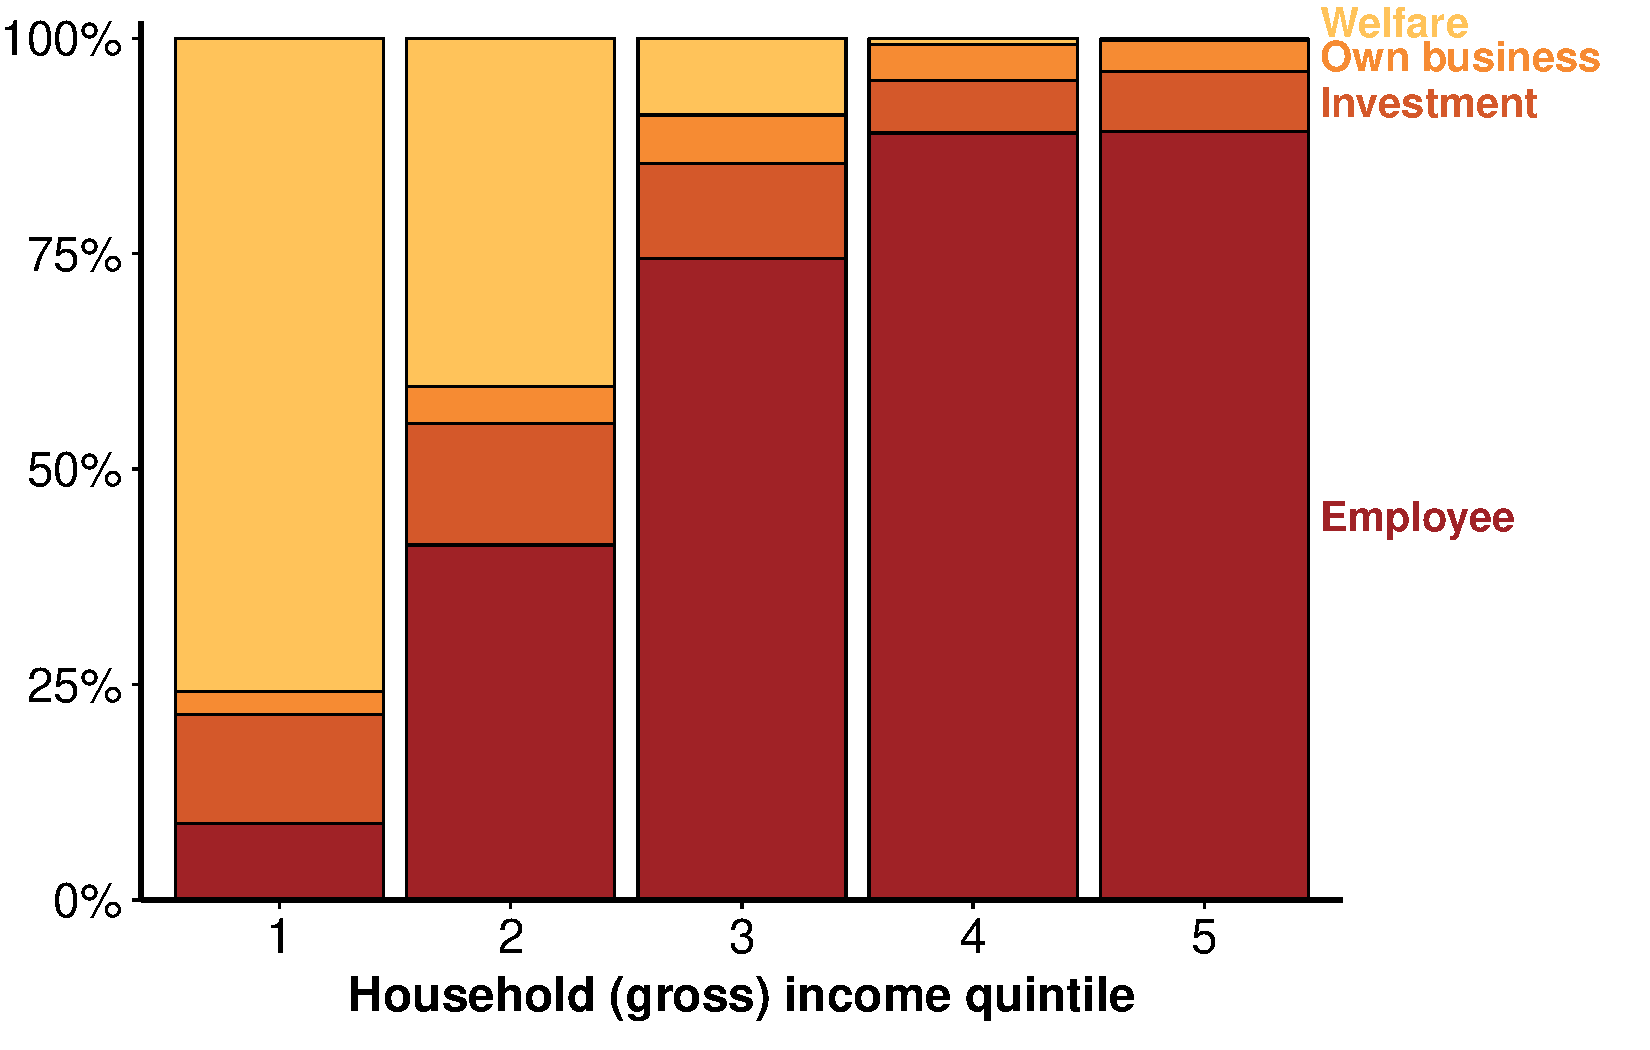
\includegraphics[width=\columnwidth]{atlas/figure/GST-Figure-5-1.pdf}
\notes{Investment income includes other income not otherwise classified. Own business income is for unincorporated businesses owned by one or more household members. Welfare includes all government payments such as pensions, unemployment benefits and family allowances.}

\source{\textcite{ABS2015HouseholdIncomeWealth1314}; Grattan analysis.}
\end{figure}

It follows that targeting compensation through the welfare system is the most direct way to compensate the poorest households. Income tax cuts will not help them much as they pay very little income tax. 

The poorest 20 per cent of households currently account for just over 10 per cent of total spending on the goods and services we have proposed to include in a broader GST and would contribute around 8 per cent of extra revenue if the GST rate was increased.\footcite{ABS2015HouseholdIncomeWealth1314}

If these households could be targeted directly, then spending 8-10 per cent of the revenues from the GST would be enough to ensure that they are no worse off on average after their higher expenses. The remaining 80 per cent of households, with higher incomes, would bear most of the net burden of the tax increase.

\begin{figure}
\captionwithunits{Higher welfare payments would also benefit some richer households\label{fig:GST-6}}%
{Average welfare payments per week by household gross income quintile, (2013-14 dollars)}
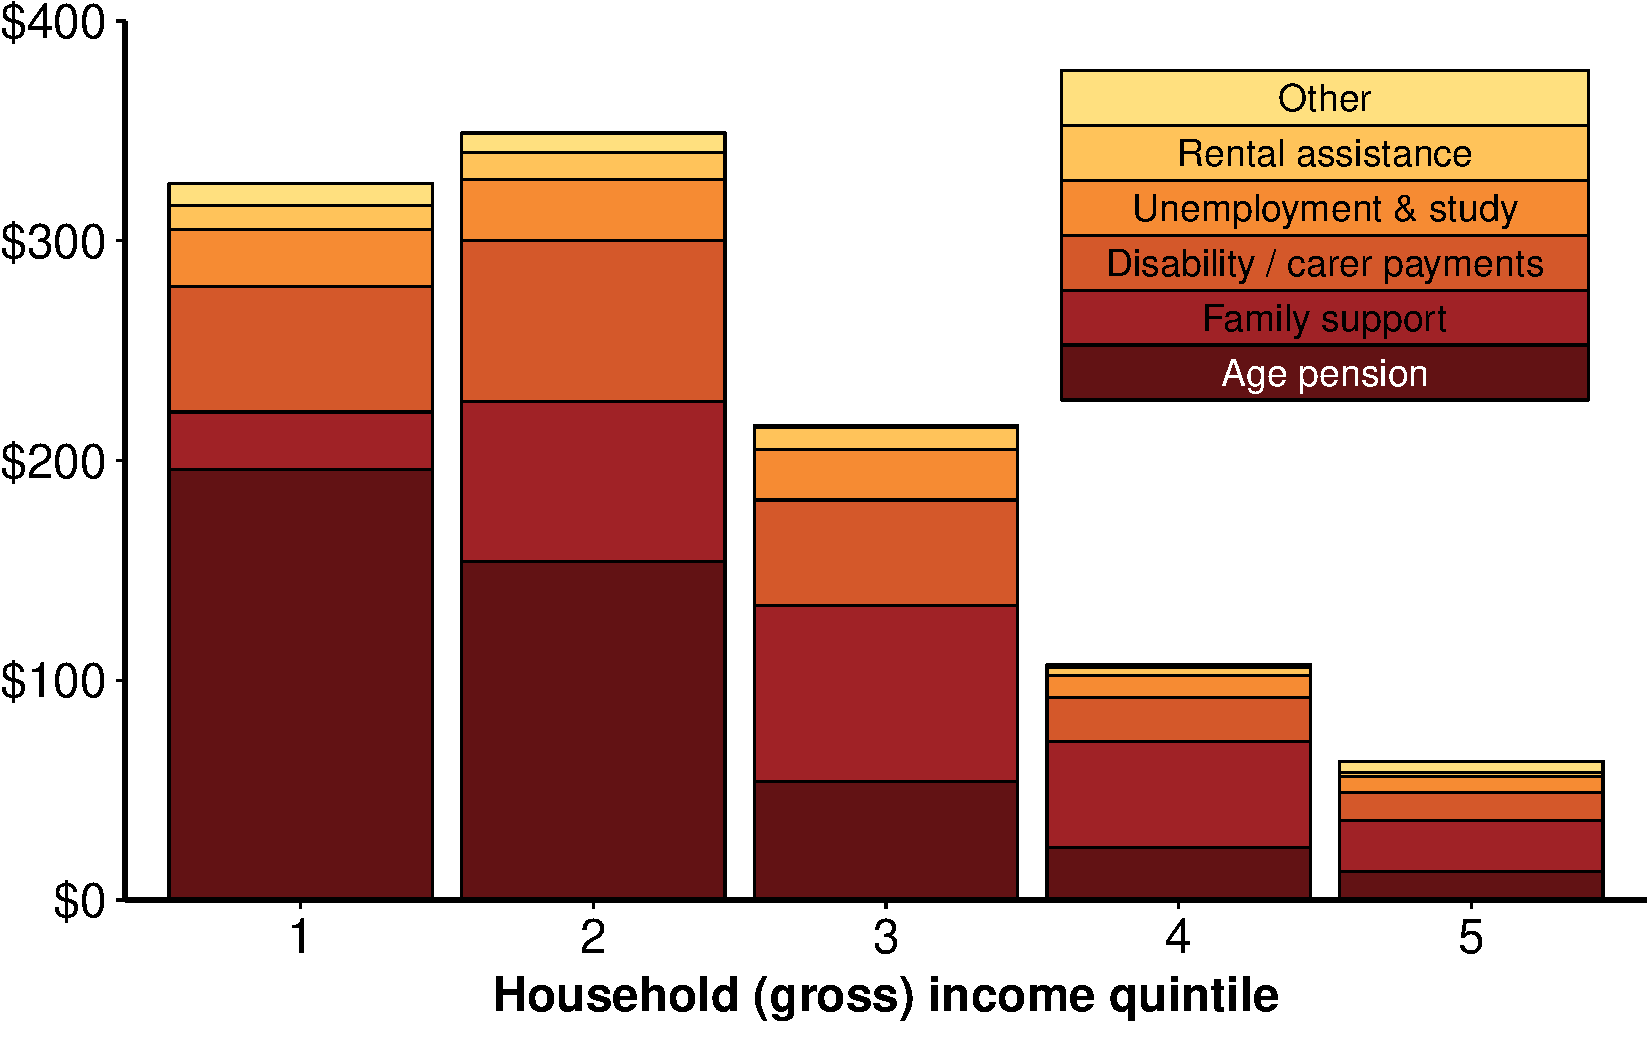
\includegraphics[width=\columnwidth]{atlas/figure/GST-Figure-6-1.pdf}
\notes{Age Pension includes Age and Veteran’s Affairs Pensions. Family payments include Family Tax Benefits and Parenting Payments.}

\source{\textcite{ABS2015HouseholdIncomeWealth1314}; Grattan analysis.}
\end{figure}

In reality, however, compensation through higher welfare payments would not be perfectly targeted. Only 30 per cent of welfare payments go to the bottom of 20 per cent of households (\Vref{fig:GST-6}). To ensure that the poorest one fifth of households are \emph{on average} no worse off, welfare benefits would have to be increased to the point where they would benefit some higher income households as well, and so would cost much more than 10 per cent of the increased GST collection. Tighter targeting would be possible if the taper rates for payments were increased, but this would substantially reduce incentives to work (\Cref{sec:GST-3-3}). 

Because low-income people also have diverse patterns of spending, it would cost even more again to provide sufficient compensation to ensure that relatively few individual households in this group would be disadvantaged by the changes. 

Given both imperfect targeting and differences in GST burden, spending around \textbf{\$8~billion}, or 30 per cent of revenues from increasing the GST rate to 15 per cent  on higher welfare benefits would ensure that the poorest households are generally more than compensated for the higher costs. A policy of overcompensation is justified because of the risk that compensation may be eroded over time (\Vref{box:GST-3}).

\begin{smallbox}{Will welfare benefits get eroded over time?}{box:GST-3}
Previous experience in both Australia and New Zealand highlights the risk that compensation can be eroded over time. Increases in welfare benefits to compensate for the introduction of New Zealand’s GST were cut sharply after a change of government.\FOOTNOTE{\textcite{Davidson2000}} In Australia, despite increases in Newstart following the introduction of the GST in 2000 and CPI indexation, the single adult Newstart rate has been eroded by cost of living increases so that it now buys less than it did before the GST was introduced.\FOOTNOTE{\textcite{ACOSS2012}}  Of course, Newstart may have been eroded even further without GST compensation.

But recent budget proposals to index pensions at inflation rather than average weekly earnings met a hostile public reaction, and were abandoned in favour of tightening eligibility for those who need pensions least.\FOOTNOTE{\textcite{Morrison2015a}}  Indeed a series of decisions over the last decade to increase pensions above average weekly earnings\FOOTNOTE{\textcite[][24]{DaleyWoodWeidmannEtAl2014}}  suggests that concerns about the longevity of compensation for pensioners may be exaggerated.

On the other hand, concerns about the value of Newstart are based on recurring political decisions to reduce payments relative to average wages. These concerns might be addressed if increases to the GST were accompanied by a substantial real increase in Newstart. Even if it were eroded over time, a large increase would leave most of those on Newstart substantially better off for some time. This might be the political price for welfare groups to support increases to the GST. 

\end{smallbox}

Distributing this money in the same proportion as existing welfare spend\footnote{We allocate compensation based on the proportion of welfare payments received by each gross income quintile. For example, 33 per cent of welfare spending goes to the second income quintile and therefore 33 per cent of new welfare spending is allocated to households on welfare in this quintile. We assume no change in the taper rates for existing payments (\Cref{sec:GST-3-3}).}  would imply substantial increases in welfare payments (\Vref{tbl:GST-1}). Effectively, the base rate of all payments would increase by around 5 per cent. \textbf{Two in three households in the bottom income quintile} would be \textbf{better off}, with more than half receiving back more than 125 per cent of their additional cost of living increases (\Vref{fig:GST-7}).

\begin{figure}
\captionwithunits{Most of the poorest households will be better off, some substantially so\label{fig:GST-7}}{Percentage of each quintile compensated by 75\%, 100\%, and 125\% of the expected price increase after higher GST and higher welfare payments}
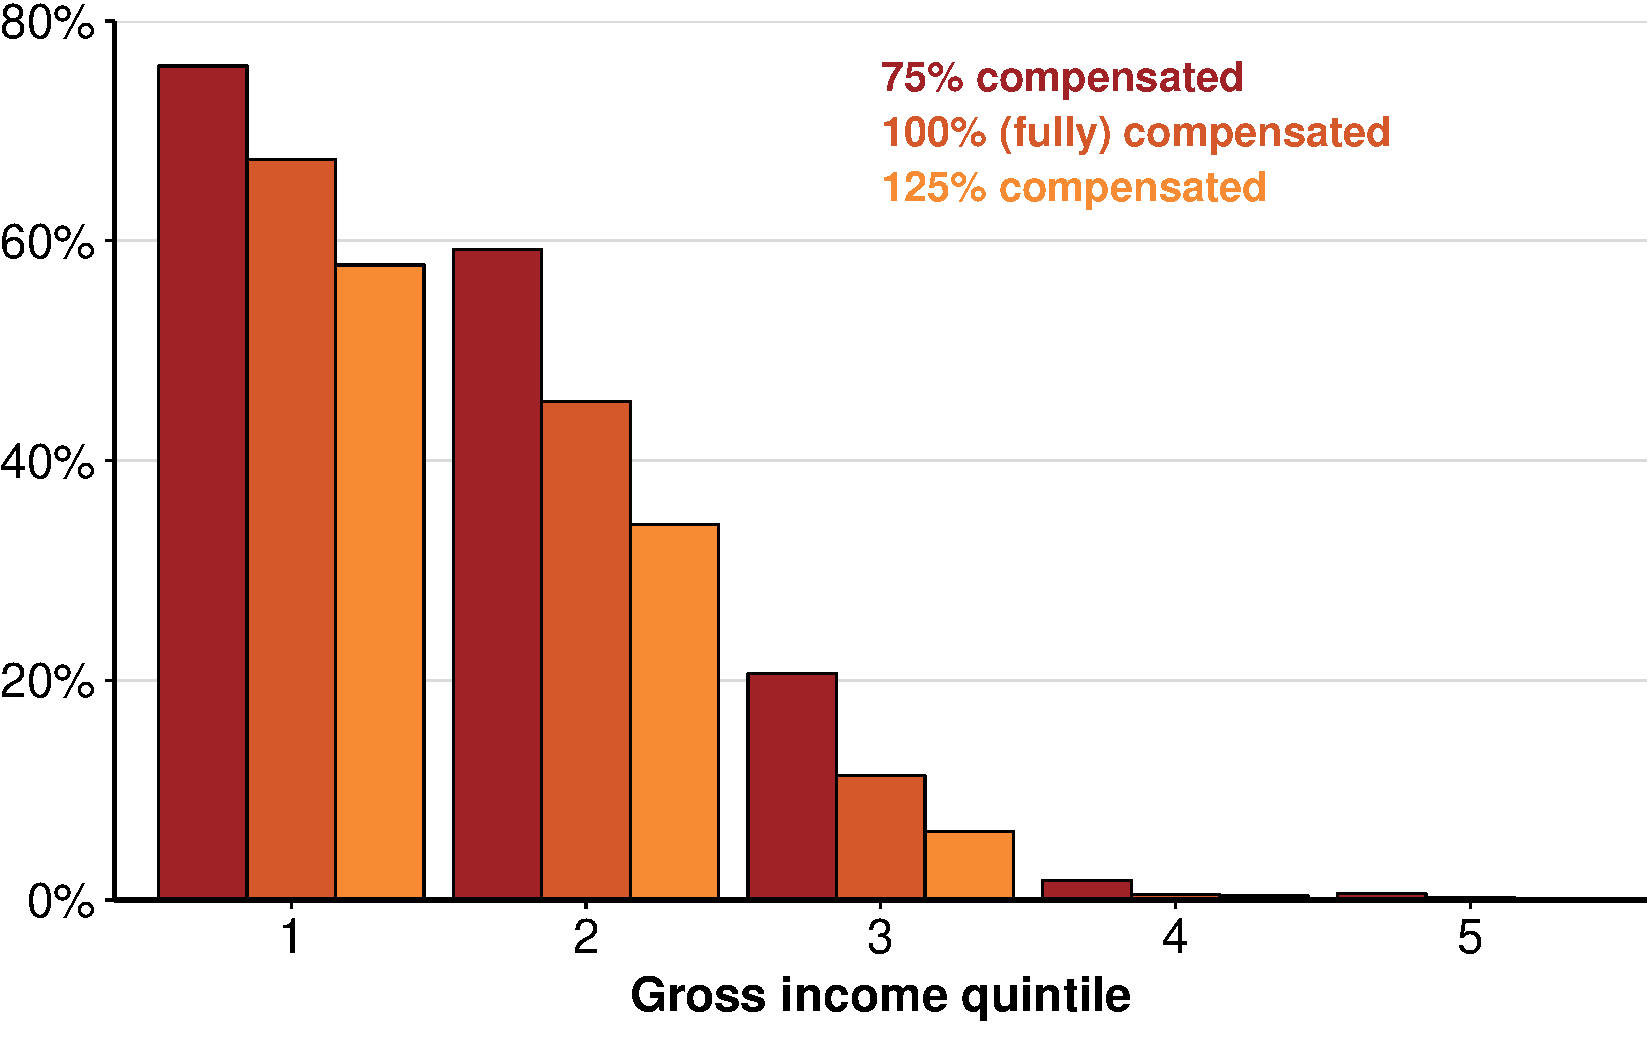
\includegraphics[width=\columnwidth]{atlas/figure/GST-Figure-7-1.pdf}
\notes{Assumes that 30 per cent of the additional revenue from increasing the GST to 15~per cent is spent on higher welfare payments. The HES understates the GST burden on households because it understates household spending. A comparison of HES with the Australian System of National Accounts (\textcite[Appendix~3]{ABS2011HES0910}), shows the difference in some spending categories – for example, tobacco, alcohol and gambling and health – exceeds 30 per cent. We inflate the HES numbers to reflect the total GST collections, assuming the downward bias in reporting is uniform across income quintiles. }

\source{\textcite{ABS2013-HES-2011-12-CURF}; Grattan analysis.}
\end{figure}

People on most full-welfare payments will be better off on average. The average single person on a full disability payment renting their home would have 1.4 per cent more to spend after accounting for their additional GST payments. While a couple of Newstart renting their home will have around 0.6 per cent more to spend. These represent modest but real improvements in the standard of living for these people (\Vref{tbl:GST-1}).

Very few people on the full rate of Newstart or the Disability Pension will be undercompensated. Around one third of full Age Pension recipients remain undercompensated, but this group is more likely to have other income sources to draw on to support higher spending (\Vref{tbl:GST-1}). 

\begin{table}
\caption{Impact of GST compensation package on selected benefits and households\label{tbl:GST-1}}
\begin{tabularx}{\columnwidth}{l>{\raggedright}XRR}
\toprule
\textbf{Benefit} & \tblHeadVCL{Household type}         & \tblHeadVC{Avg. change in\\disposable\\income (\%)} & \tblHeadVC{Proportion under-\\compensated} \\
\midrule
Full Age pension & Couple, home-owners             & 0\%                                           & 36\%\\[1.5\baselineskip]
Newstart         & Couple, 2 children, renters     & 0.8\%                                         & 9\% \\[1.5\baselineskip]
Disability       & Single, no other income, renter & 1.4\%                                         & 21\% \\[1.5\baselineskip]
\bottomrule
\end{tabularx}
\notes{This analysis is based on welfare benefits and spending patterns from 2009-10 because this is the most recent year for which spending data at the household level is available.}

\source{Grattan analysis.}

\end{table}

Changes that over-compensated most households on Newstart would recognise the substantial financial distress of these households,\footcite[][18--19]{DaleyMcGannonEtAl2013}  and the possibility that higher payments may increase workforce participation by making it easier for individuals to present themselves well or to maintain their readiness for work.  There is a broad consensus amongst welfare groups, economists and business lobbies that Newstart payments are too low.\footcite[][3]{BCA2012}  The rising gap in living standards between those receiving Newstart (and other allowances) and those receiving a pension is due to less favourable indexation for Newstart.\footnote{Newstart and family payments are indexed to the CPI, which means they increase to keep pace with movements in prices but not community living standards. In contrast, pensions (including age, disability \etc) are indexed to Male Total Average Weekly Earnings (MTAWE) or CPI/the Pensioner and Beneficiary Living Costs Index (an alternative price index), whichever is highest. \textcite{DSS2015}. }  

This analysis overestimates how many people in the bottom quintile would be worse off. The ABS survey used for calculating the impacts of taxes appears to have a substantial number of households that misstate their income. About 0.6 per cent of all households (by definition in the bottom quintile) are recorded in the ABS survey as having zero or negative income, and another 1.9 per cent have incomes less than Newstart for a single person of \$11,682 per year (2009-10). Despite their very low incomes, these households spend on average as much as households in the second income quintile. If all these households have incomes reflecting their spending, then 73 per cent of the lowest income quintile would be fully compensated by our proposed package, rather than 67 per cent as shown in \Vref{fig:GST-7}.\footnote{The spending pattern of these households more closely resembles that of the second income quintile than the lowest.}

Inevitably some poorer households will not be fully compensated. This is an unfortunate reality of any revenue-positive tax reform. Increasing welfare payments to ensure that \emph{no one} on low incomes is worse off – in terms of spending power – would substantially increase the cost of the package. But reform should not require that \emph{no one} goes backwards. Some in the bottom 20 per cent will be losers; many more will be winners. 

Our analysis of the lowest 30 per cent of people at the bottom of the income distribution who would be undercompensated does not identify any one particular group systematically disadvantaged by the proposals. Those left worse off by the compensation package are spread across the age distribution and include people receiving welfare as well as people reliant on private income. Almost half of the low-income earners not fully compensated have net wealth of more than \$500,000.\footnote{\gao\ \textcite{ABS2013-HES-2011-12-CURF}.}  Some could be business owners or investors who have understated their income. Some are probably households, such as part-pensioners, drawing down on their assets to finance consumption. 

The fact that some people will be slightly worse off will make reform politically harder, but there is no principled reason to preserve the precise rank order that applies today to those in the bottom 20 per cent.

In any case, it is reasonable to ask that some on lower incomes – just like others in the population – contribute to paying for the improvements in government healthcare which that benefit them,\footcite[][14]{Deloitte2015TaxReformSheddingLight}  but come at a growing cost to budget bottom line.\footcite[][20]{DaleyWoodWeidmannEtAl2014}  Improvements in access to or quality of health services funded by the GST will provide benefits to all Australians. These benefits are in addition to the financial compensation modelled in this paper.

\section{Increased welfare payments can be designed so there is little effect on work incentives\label{sec:GST-3-3}}
Compensation can be structured so that incentives to work do not change much. If welfare payments are increased by a fixed amount, but the rates at which benefits reduce (as incomes go up) do not change, then effective tax rates for current welfare participants are also unchanged (\Cref{box:GST-4}).

The main impact on work incentives will be for those people brought into the net for welfare benefits. These people will face higher effective marginal tax rates as any additional income they earn will result in the loss of some welfare benefits. However, our estimates suggest this group is relatively small – the package might add about 10,000 Newstart recipients to the 680,000 who currently receive this payment (\Cref{box:GST-4}).%
\footnote{We assume that the additional welfare in our package (totalling approximately 5 per cent of current welfare spending) increases all payment categories by an equal percentage. The number of additional individuals who would receive the Newstart allowance is given by the number of individuals without welfare payments whose taxable income is between 100 per cent and 105 per cent of the current maximum income for Newstart recipients.}   

\begin{bigboxC*}{Structuring welfare payments to reduce disincentives for work}{box:GST-4}
%\setlength{\parskip}{11pt}
Means tested welfare payments reduce work incentives. If welfare recipients start earning income, they not only pay tax on each dollar of income earned but also forego some of their benefits. The impact on work incentives is moderated by a ‘taper’ which reduces benefits gradually as incomes increase.

If the same ‘taper’ is maintained, then higher welfare payments have little impact on incentives to work. If welfare increases by a fixed dollar amount for all recipients (whether they are receiving a full or part benefit) then there is no change to the taper. For almost all levels of income, the dollar value of payments withdrawn with each additional dollar earned is the same under the new compensation arrangements (\Cref{fig:GST-8}). 

By contrast, a proportional increase in benefits would make the taper rate steeper, increasing effective tax rates for those on particularly low incomes.

However, even a fixed dollar increase in benefits will have some effects on incentives to work.  

First, because higher welfare payments will increase real income for some recipients, this could make working less attractive relative to welfare benefits. However, it is not clear this effect will be substantial given that the proposed increase in payments is relatively small, and welfare payments will generally remain well below wage levels. 

\begin{figure}[H]
\captionsetup{format=plain,font={small,bf,theGrey},labelfont={small,bf,theGrey}, justification=raggedright,
singlelinecheck=false,position=top,skip=0pt}
\caption{A fixed dollar increase in welfare payments maintains the marginal incentive to work\label{fig:GST-8}}
% \begin{scaletikzpicturetowidth}{\linewidth}
\begin{tikzpicture}[x=0.9\linewidth, y = 0.5\linewidth]
\tikzstyle{every node}=[font=\small, text badly ragged]
    % Draw axes
    \draw [thick, color=theGrey] (0,1) node (yaxis) [above, align=left] {} |- (1,0) node (xaxis) [below, align=right] {};
    \node[anchor=south west, rotate=90] (ylab) at (0, 0.1){\color{theGrey}Benefits (\$) $\longrightarrow$};
    \node[anchor=north west, rotate=00] (xlab) at (0.06666, 0){\color{theGrey}Income earned (\$) $\longrightarrow$};
 	% Draw lines
 	\path[draw, line width = 1.5pt, color=Color3] (0, 0.70) -- (0.15, 0.70) node (A){} -- (0.65, 0) node (B){};
 	\path[draw, line width = 1.5pt, color=Color5] (0, 0.80) -- (0.15, 0.80) node (A1){} -- (0.7214286, 0) node (B1){};
    % Draw two intersecting lines
    \node (CC) at ($(A)!0.5!(B)$) {};
    \node (DD) at ($(A1)!0.5!(B1)$){};
    \node[text width = 2.5cm, align=flush right, node distance=5pt] (CClab) at (0.10, 0.2) {\color{Color3}Current\\ compensation\\ arrangements};
    \draw[-latex, line width = 1pt, color = Color3, node distance = 5pt] (CClab) edge[in=-135, out=0] (CC);    
    \node[text width = 2.5cm, align=left, node distance=5pt] (DDlab) at (0.75, 0.65) {\color{Color5}Compensation\\ post-GST};
    \draw[-latex, line width = 1pt, color = Color5, node distance = 5pt] (DDlab) edge[out=180, in=45] (DD);
    %
    \draw[-latex, line width = 1pt] (0.15, 0.90)node[anchor=south west, inner sep = -2.5pt, align=left, text width = 2.5cm]{Fixed \$ increase \\ \quad in benefits} -- (0.15, 0.8);
    \draw[-latex, line width = 1pt] (0.15, 0.60) -- (0.15, 0.7);
    %
    \node[inner sep = 0pt] (B1b) at (0.7214286, -0.04){};
    \node[inner sep = 0pt] (Bb)  at (0.65, -0.04){};
    \node[anchor=north west, inner sep = 0pt, align=left, font={\bfseries\small}] (Bblab) at (0.65, -0.08){ People on higher incomes\\ brought into welfare net};
    \draw[->, line width = 2pt, inner sep = 0pt] (Bb) -- (B1b);
\end{tikzpicture}
\end{figure}
% TODO: Should there be reduced space here

Second, some people will face higher EMTRs because they are brought into the welfare net. People on incomes a little above the previous cut off point will now receive a (modest) welfare benefit (\Vref{fig:GST-8}). This increases their effective tax rate because they will now forego this benefit as their income increases. However, the number of people affected is modest – we estimate, for example, that with the compensation we propose, an extra 10,000 people might qualify for some Newstart payment, a small number relative to the 680,000 or so that currently receive Newstart. 


\end{bigboxC*}

\section{Income tax cuts can compensate the average lower income household\label{sec:GST-3-4}}
Modest income tax cuts should be part of a GST reform package.

Appropriately targeted income tax cuts will help to moderate the effect of a higher GST on work incentives. By increasing the prices of many good and services, a higher or broader GST reduces the real purchasing power of take home pay. But income tax cuts mean that workers will have bigger pay packets. 

This partial ‘swap’ of income taxes for consumption taxes will provide an economic dividend. However, the economic gain will depend on the design of any income tax cuts: cuts targeted at low and middle income earners are likely to increase workforce participation more than reductions in the top marginal rate only paid by a small number of taxpayers who usually work full time (\Vref{box:GST-5}). 

\begin{smallbox}{Impact of taxes on labour supply}{box:GST-5}
There is a comprehensive literature on the effect of taxes on labour supply decisions. Two review papers – \textcite{MeghirPhillips2008} and \textcite{CBO-2012-Labor-Supply-Elasticity} \textcite{CBO-2012-Labor-Supply-Elasticity} – summarise this work and nominate the findings for which there is consensus or near consensus.

Their conclusions are broadly consistent. Almost all the studies referenced find that men’s hours of work are unresponsive to tax changes. This is because most men work full time. But for men with low levels of education, the decision of whether to work is somewhat affected by tax and welfare incentives (\textcite{MeghirPhillips2008}). For highly educated men, tax rates make almost no difference to work decisions. But tax rates do affect their taxable incomes: high-income taxpayers are more likely to convert income into more lightly taxed forms – such as capital gains – when tax rates are high (\textcite{MeghirPhillips2008}). They are also able to respond by shifting their income into a period when their tax rates are lower – such as retirement (\textcite{CBO-2012-Labor-Supply-Elasticity}).

On the other hand, empirical studies invariably find that tax and welfare benefits have a much greater bearing on working decisions for women with young children: they affect both the decision to work and the number of hours worked. However, the CBO paper finds the responsiveness of women’s labour supply decisions in the US is falling as their workforce attachment grows.

Taken together, these studies suggest that tax rates have the most effect for people on low and middle incomes deciding whether to work or whether to increase their hours. If one objective of tax reform is to increase workforce participation, then tax cuts should focus on the low to middle brackets.

\end{smallbox}


While some argue that cuts at the upper end should be prioritised to spur entrepreneurial activity,\footnote{For example, Graeme Bradley, former Business Council of Australia president, cited in: \textcite{BaloghHepworth2015}. See also: \textcite{Hockey2015d}.}  our tax system already provides numerous incentives for starting a business, such as deductibility of losses, a 50 per cent discount on capital gains income and a host of small business capital gains exemptions.\footnote{Exemptions from capital gains tax for small business owners include: 
 exemptions for the sale of active assets (needs to be paid into a super fund for people under 55); and an exemption for people over 55 who are retiring and selling business assets held for more than 15 years. A lifetime cap of \$1.4 million applies to these exemptions. See: \textcite{ATO2014f} as well as \Cref{part:SUPER} at \pageref{paragraph:SUPER-lifetime-CGT-cap}.
}  

If the purpose of GST reform is to reduce future deficits, to fund reductions in taxes that drag more on economic growth, or to help state governments fund rising healthcare costs, there is a limit to the money available to fund income tax reductions. Given our proposed welfare package, spending any more than 30 per cent of the revenue on income tax cuts would not leave enough funds to make a meaningful dent in deficit reduction, tax reform or the future health funding ‘gap’. 

We propose a package of income tax cuts that helps protect the welfare of lower and middle income households. Spending 30 per cent of additional GST revenues allows for modest income tax cuts in the low to middle brackets. 


For example, using \$8 billion of the additional \$27 billion of revenue from a 15 per cent GST would allow a reduction in the bottom tax bracket from 19 per cent to 16.5 per cent and a reduction in the next bracket from 32.5 to 30.5 per cent. If, instead the GST is broadened, 30 per cent of the revenue from a broader GST would support cuts to approximately 17.5 per cent and 31.5 per cent for the same brackets (\Vref{tbl:GST-2}). To put them in context, these tax cuts would have a similar impact on average tax rates as three to five years of forecast bracket creep.  Households higher up the income scale would also receive substantial benefit from these tax changes. 

\begin{table}
\caption{Proposed income tax cuts\label{tbl:GST-2}}
\begin{tabularx}{\columnwidth}{l@{}c@{}rRRR}
\toprule
\multicolumn{3}{l}{\begin{tabular}[b]{@{}l@{}} \multirow{2}{*}{\textbf{Tax bracket}}\end{tabular}} & \textbf{Current tax rate} & \textbf{Rates with higher GST} & \textbf{Rates with broader GST} \\
\midrule
%
\$0& \ -- \  &\$18,200 & 0\% & 0\% & 0\% \\[0.5\baselineskip]
\$18,201& \ -- \  &\$37,000 & 19\%\ & 16.5\% & 17.5\% \\[0.5\baselineskip]
\$37,001& \ -- \  &\$80,000 & 32.5\% & 30.5\% & 31.5\% \\[0.5\baselineskip]
\$80,001& \ -- \  &\$180,000 & 37\% & 37\%\ & 37\%\ \\[0.5\baselineskip]
\multicolumn{3}{l}{\$180,000 and over} & 45\% & 45\% & 45\% \\[0.5\baselineskip]
\bottomrule
\end{tabularx}
\notes{Excludes Temporary Budget Repair Levy (2\% for those earning over \$180,000 until 2016-17).}
\end{table}

\Cref{fig:GST-9} shows the combined effect of our package with a higher GST, lower income tax rates and higher welfare payments.

\begin{figure}
\captionwithunits{Welfare increases and income tax cuts would offset higher GST for most lower-income households\label{fig:GST-9}}%
{Percentage of each quintile compensated by 75\%, 100\%, and 125\% of the expected price increase after higher GST and higher welfare payments}
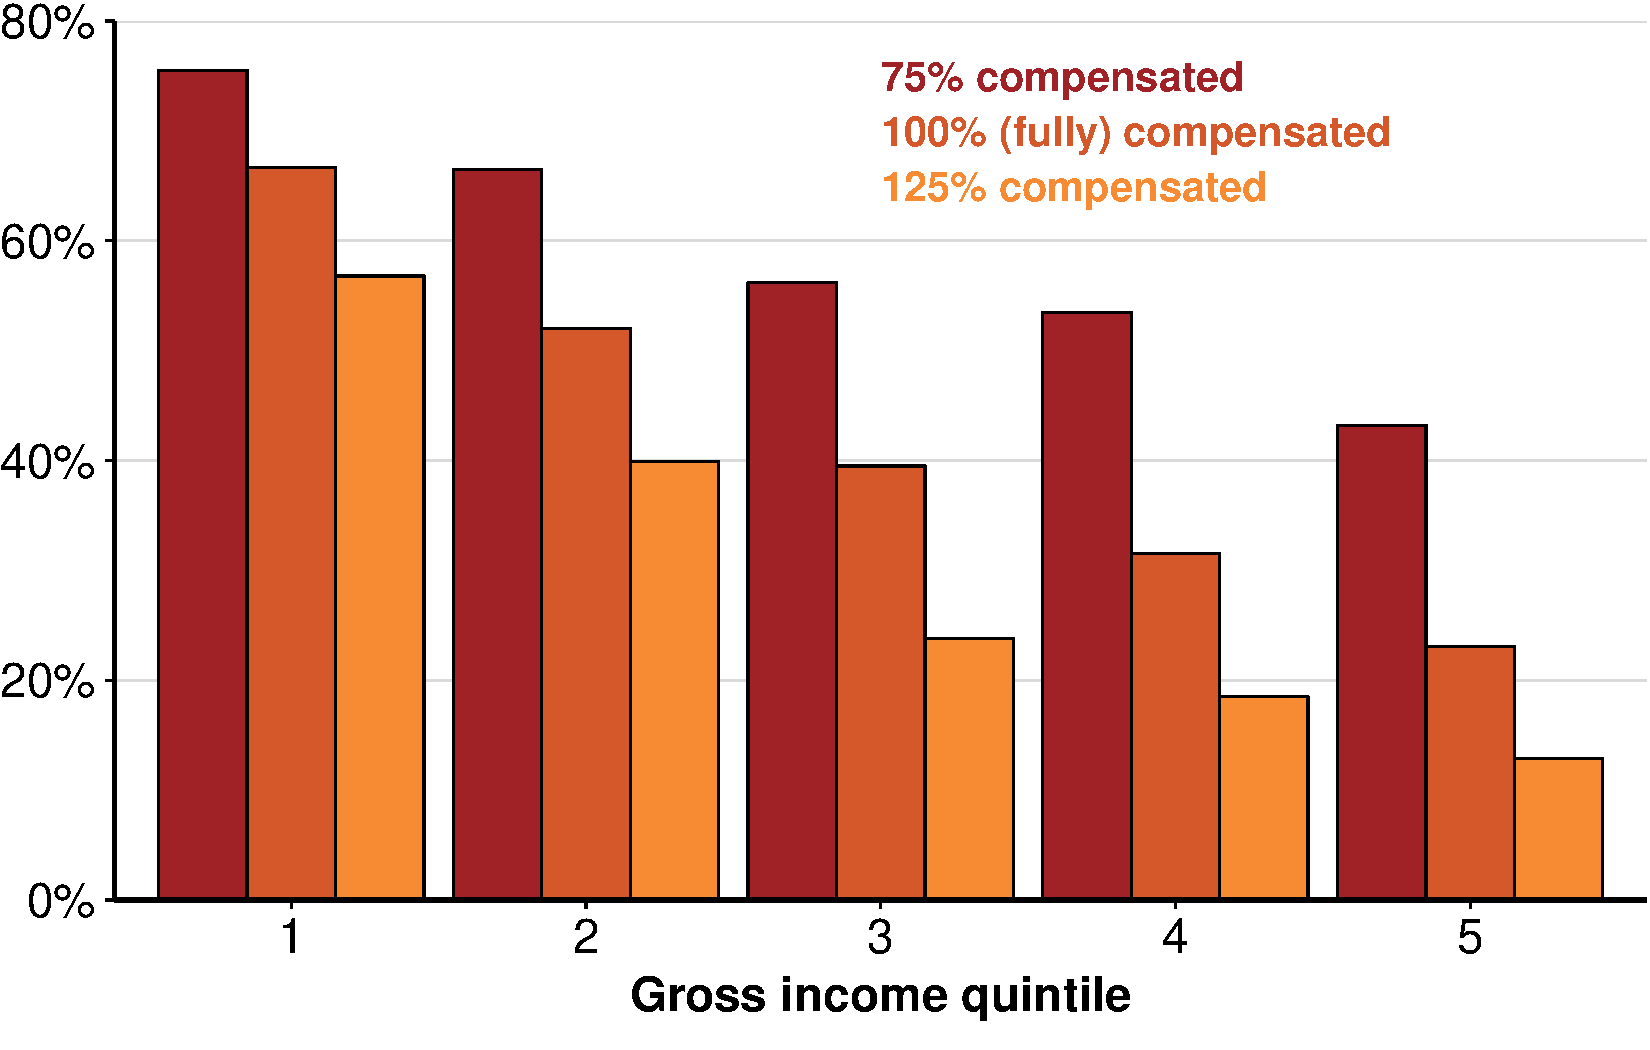
\includegraphics[width=\columnwidth]{atlas/figure/GST-Figure-9-1.pdf}
\notes{Assumes that 30 per cent of the additional revenue from increasing the GST to 15 per cent is spent on higher welfare payments and an additional 30 per cent is spent on tax cuts. Tax cuts applied to the 2009-10 survey respondents. Magnitude of the cuts to the marginal rates calibrated to result in a change in revenue of approximately 30 per cent of the contemporaneous GST revenue. See also note to \Cref{fig:GST-7}.}

\source{\textcite{ABS2013-HES-2011-12-CURF}; Grattan analysis.}
\end{figure}

Most households in the bottom 40 per cent – with incomes up to \$63,000 annually\footnote{This was the maximum income for a household in the bottom 40 per cent of household incomes in 2013-14. See: \textcite{ABS2015HouseholdIncomeWealth1314}.}  – would come out in front under our package. Middle and upper middle income households on average would come out behind, but not by much: lower income taxes and higher welfare payments would offset three quarters or more of the effects of a higher GST for households in the third and fourth income quintiles (\Cref{fig:GST-9}). The average fall in disposable income for these households is 0.6 per cent.\footnote{\gao\ \textcite{ABS2013-HES-2011-12-CURF}.}  

\begin{table}
\caption{Budgetary impact of income tax rate changes}\label{tbl:GST-3}
\begin{tabularx}{\columnwidth}{lr>{\raggedleft\arraybackslash}X}
\toprule
\tblHead{Tax bracket} & \tblHead{Current tax rate} & \tblHeadR{Budgetary impact of 1~percentage point change, billions (2015-16)}\\
\midrule
\$0-\$18,200 & 0\% & \\
\$18,201 - \$37,000 & 19\% & \$1.9\\
\$37,001 - \$80,000 & 32.5\% & \$2.3\\
\$80,001 - \$180,000& 37\% & \$1.3\\
\$180,001 + & 45\% & \$0.7\\
\bottomrule
\end{tabularx}
% TODO: brackets need to be consistent
\end{table}

Of course, other changes to income tax rates would distribute the benefits differently, with different costs to the budget, as shown in \Vref{tbl:GST-3}. 

Politicians might be tempted to try to fully compensate all low- and middle-income households. But because GST affects different households in very different ways, it is extremely expensive to ensure there are no losers. Tax cuts to fully compensate almost every household earning up to \$100,000 for a 5 per cent increase in the GST would have cost approximately \$23.5 billion in 2012 13 – and this would be an underestimate of the budgetary impact today.\footnote{This is based on compensating 80 per cent of households in the third income quintile (and more with lower incomes). The income of the 60th percentile household was approximately \$100,000 in 2013-14. See: \textcite{ABS2015HouseholdIncomeWealth1314}. The analysis assumes household income is earned by a single income earner. Households earning up to \$100,000 split between more than one income earner would require even larger tax cuts for equal compensation.}  This would be in addition to the \$8 billion in additional welfare payments required to compensate the most vulnerable (\Cref{sec:GST-3-2}). Together, the amount spent on compensation, in excess of \$30 billion, would exceed the additional \$27 billion in revenue collected. It is simply not possible to fully compensate most households this far up the income distribution with a package that doesn’t increase budget deficits.

There will also be calls to find ways to compensate those that fall outside of the tax and transfer net. The largest and most vocal group in this category are self-funded retirees. When the GST was introduced in 2000, self-funded retirees received one-off cash payments – a savings bonus and a self-funded retiree bonus worth up to \$3000\footcite{GST-Act-Bonuses-for-Older-Australians-1999}  – to compensate them for the higher cost of living associated with the GST. 

Such payments are expensive – the estimated impact in 2000-01 was \$1.3 billion and would be much higher now for an equivalent package – and not justified. Self-funded retiree households are not amongst the vulnerable: there are few self-funded retirees in the poorest 20 per cent of Australians households. Any retirees with incomes at this level would qualify for at least a part-pension. Nor can the payments be justified on the grounds of fairness, given that self-funded retirees currently pay far less tax than a working household on the same gross income.\footnote{Self-funded retirees pay no tax on any earnings within their superannuation accounts or on any draw-downs from these accounts. See: \Cref{part:SUPER}.}  

\chapter{The uses of GST revenue}\label{chapter:GST-4}
If the GST is broadened or raised, governments will have additional revenue of between \$7 and \$11 billion a year after paying for the compensation package we have proposed. This additional revenue might:
\begin{itemize}
\item	reduce the hospital funding ‘gap’ of state governments;
\item 	reduce the Commonwealth’s substantial deficit; 
\item 	fund other tax cuts, over and above the income tax cuts focused on the lower thresholds proposed as part of the compensation package. 
\end{itemize}
The federal politics are likely to require that at least some of the GST revenue improves the net budget position of the states and territories. Ultimately, it will be necessary to broker a deal that will be acceptable to both Commonwealth and states. States are unlikely to be enthusiastic about surrendering the principle that all GST revenue is transferred to them. So the Commonwealth will also need to reduce tied grants to fund the compensation package. 

\section{Some of the GST increase will need to go to state governments}\label{sec:4-1}
State and Territory governments are likely to demand a sizeable share of additional GST revenue as a minimum price for their cooperation. This would consume a substantial portion of the additional revenue raised by changes to the GST, net of the compensation package.

Government health spending in Australia – and in developed countries around the world – has consistently grown much faster than the economy over the last 20 years.\footcites[][25--27]{DaleyWoodWeidmannEtAl2014}[][17]{DaleyMcGannonHunter2014}  And while there is clearly scope to reduce costs in parts of the system,\footcites{DuckettBreadonGinnivanEtAl2013}{DuckettBreadonRomanesEtAl2015}  there have been apparent dividends from higher spending – life expectancy and years lived free from disability have increased.\footcite[][16]{Daley2015}  

Under the Council of Australian Governments National Health Reform Agreement, the Commonwealth agreed to share the costs of efficient growth in hospital activity, initially meeting 45 per cent of the cost growth, rising to 50 per cent in 2017.\footcite[][13]{COAG2011}  However, under changes announced in the May 2014 budget, the Commonwealth announced that its support for state health spending would only grow in line with inflation and population growth – far below the expected growth in health spending.\FOOTNOTE{See \Vref{sec:FISCAL-4-3}.}  State governments would have to fund all increases in real spending per person for hospitals.\footcite[][Budget Paper No.~2, p.~126]{Treasury2014-Budget-Papers-2014-15}  

This decision will have a large and growing impact on state government budgets. The Commonwealth estimates that by 2024-25 the changed policy will reduce its nominal transfers to the states for hospitals by around \$15 billion.\footcite[][115]{SenateEconomicsLegislationCommittee2014}  By 2054-55, the reduction in spending for hospitals will be many times larger.  Similar policy decisions in schools funding will reduce nominal Commonwealth spending on schools by \$6 billion by 2024-25.\footcite[][115]{SenateEconomicsLegislationCommittee2014}

States are unlikely to cooperate with changes to the GST unless the changes make a material net contribution to state budgets. Although the GST legislation technically requires the consent of all states and territories for amendments to the rate or base,\footcite[][\S11]{GST-Act-Rate-Base-1999}  the Commonwealth Parliament can ignore this requirement, by simply repealing the section requiring state and territory consent.\footcite{Twomey2003}  Nonetheless, it would be politically unwise for the Commonwealth to pursue reforms without substantial state government support. But without some net contribution to their budgets, it is difficult to see why state governments would cooperate with the Commonwealth to increase the GST, considering all the political costs such support would entail. 

The minimum price for a deal is likely to be around \$5 billion a year – roughly half the health funding withdrawn by the Commonwealth by 2021-22,  and roughly half the additional revenue available after compensation if the GST is raised to 15~per~cent.

\section{GST increases could also reduce the Commonwealth's substantial deficit}\label{sec:GST-4-2}
Any additional GST revenue could go to reducing the Commonwealth’s substantial deficit. The Commonwealth has posted structural deficits for the last 8 years.  Based on current policies, these deficits are likely to continue. Projections that show these deficits being reduced quickly over the next four years of the forward estimates seem optimistic.  Budget repair will almost certainly require both tax increases and spending reductions.\footnote{See \Vref{chapter:FISCAL-2}, also Martin Parkinson cited in \textcite{Uren2015-Parkinson-tackle-spending-revenue}.}  Tax increases through the GST are likely to distort economic activity less than most of the alternatives, and definitely less than bracket creep, which is the dominant driver of the Commonwealth’s planned return to surplus.  Half of the available additional revenue from raising the GST to 15 per cent – \$5~billion a year  – would reduce the Commonwealth’s budget deficit by around 15 per cent.\footnote{Commonwealth deficit for 2015-16 estimated at \$35.1 billion. \textcite{Treasury2015FinalBudgetOutcome1415}.} 

\section{GST increases could also fund other tax reductions}\label{sec:GST-4-3}
The additional GST revenue could instead fund other tax reductions, including further income tax cuts,\footnote{Scott Morrison as quoted in \textcite{Coorey2015a}.}  cuts to corporate taxes,\footcite{FinancialServicesCouncil2015-Tax-white-paper-submission}  or state stamp duties.\footcite{PropertyCouncil2015-Tax-reform}  The relative merits of these proposals are beyond the scope of this paper. Roughly speaking, additional revenue of \$5 billion from the GST could fund:
\begin{itemize}
\item	a reduction in marginal income tax rates of close to one percentage point for every bracket\footnote{A full one percentage point cut to all brackets would cost around \$6.2~billion, see: \Vref{tbl:GST-3} on the budgetary costs of income tax rate changes.}  (this would be in addition to the cut in income tax rate for the lower two brackets described in \Cref{sec:GST-3-4}); 
\item 	a general cut of 2 to 3 percentage points for corporate taxes;\footnote{Approximate figure based on the tax rate that would reduce the \$68~billion in company tax collections in 2014-15 by approximately \$5~billion. The \textcite{BusinessTaxWorkingGroup2012} released a discussion paper that estimated a \$5 billion cost to revenue (before dynamic changes such as increased activity) from a 3 percentage point cut to company tax. Company tax receipts are at a similar magnitude currently to what they were at the time of that estimate. See: \textcite[][Statement~4]{Treasury2015BudgetPapers201516}.}  or
\item 	a cut in the rate of state stamp duties by a third.
\end{itemize}
\section{Federalism makes introducing such a package more challenging\label{sec:GST-4-4}}
A package that raises GST collections and delivers enough to all governments involved would shake up existing federal-state financial relations. 
Raising the GST will impose political costs on both Commonwealth and state and territory governments. Such a reform would require – as a matter of political reality – the support of the Commonwealth Government and a majority of the state governments. This support is unlikely unless both the Commonwealth and state and territory governments achieve a net benefit. 

But a politically plausible compensation package for increasing the GST to 15 per cent, such as that described in \Cref{chapter:GST-3}, would effectively cost the Commonwealth budget \textbf{\$16 billion} a year – \$8 billion in tax cuts and \$8 billion in higher welfare payments – if it did not pocket any of the revenue. 

There are different ways the Commonwealth could fund this cost. 

The Commonwealth could retain a portion of the GST collected. But the states and territories will be reluctant to abandon the current principle that the Commonwealth passes on all of the GST it collects. Any sign that the Commonwealth intended to retain some of the GST revenue would probably be seen by the states as the thin end of the wedge  unless it was part of a ‘big bang’ reform to federal-state relations such as the one proposed recently by the South Australian premier.  Having got its hands on some GST, it would be very tempting for a cash-strapped Commonwealth to retain a bigger portion in the future. The states and territories would be right to be suspicious: the Commonwealth has a long track record of reducing grants to the states when it faces budget pressures, effectively transferring Commonwealth budget problems to the States.

Alternatively, the Commonwealth could reduce some of the tied grants that it provides to the states, while commensurately increasing untied GST funding.\footnote{It would be possible to phase in this transition over time – with additional funding initially tied based on the existing profile of tied grants but converting to untied funding.}  Many state governments would find this attractive, so long as they received a material increase in funding overall as an incentive for their cooperation. Indeed, delivering the states greater autonomy in the service areas where they have jurisdiction is seen as important objective of reform to federal-financial relations.\footnote{The Issues Paper for the White Paper on Reform to the Federation points to accountability for performance as one of the key issues to be considered in reforming the federation \textcite[][13--25]{PrimeMinisterCabinet2014a}.}  

However, it is likely to meet political opposition. Lobby groups would be reluctant to see tied-payment funding earmarked for their policy area converted to untied funding that states might choose to spend elsewhere. For example, independent school groups are likely to oppose a reduction in tied grants for independent school funding even if there is a commensurate increase in untied funding. They would fear that State governments might subsequently reduce funding to independent schools.

The scale of funding involved exacerbates the problem. If the States insist on continuing to receive the entirety of GST collections as untied grants, then the Commonwealth would need to reduce tied grants by around \$22 billion a year if the GST rate is increased to 15 per cent.\footnote{This assumes that the states receive a net increase in funding from the package of \$5 billion a year to offset the historic reduction in Commonwealth tied funding for health.}   This would offset the hits to the Commonwealth budget from the compensation package as well as providing some improvement to Commonwealth revenue collections.

Commonwealth transfers to the states will total \$108 billion in \mbox{2015-16} of which \$50~billion are for tied grants. A reduction in tied grants of \$22 billion a year would require the Commonwealth to untie funding for either of schools or hospitals, or all other areas (\Vref{fig:GST-10}). 

\begin{figure}
%% Figure 
\captionwithunits{Cuts to tied grants would need to occur in politically sensitive areas\label{fig:GST-10}}%
{Commonwealth transfers to states by sector, billions, 2015-16}
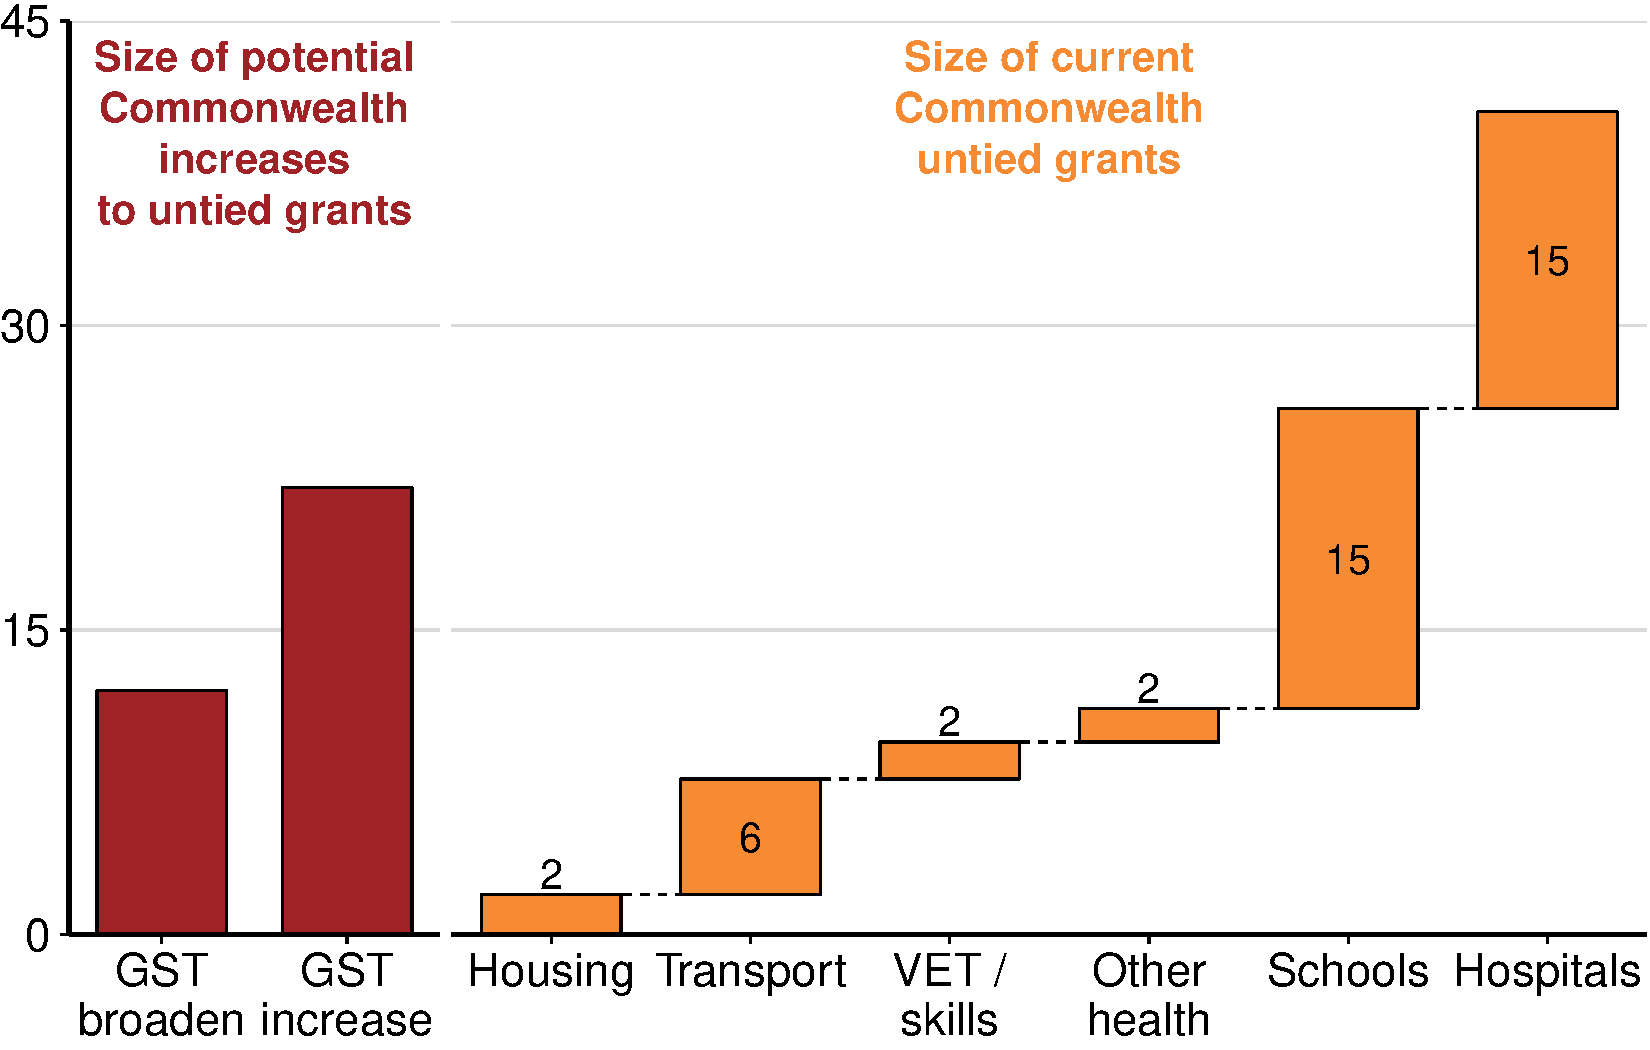
\includegraphics[width=\columnwidth]{atlas/figure/GST-Figure-10-2.pdf}
\source{\textcite[Budget~paper~3, Table~2.2]{Treasury2015BudgetPapers201516}.}
\end{figure}

But these challenges are not insurmountable. Over time giving states greater control over their spending will arguably improve efficiency and accountability\footnote{ A number of concerns have been raised about the way tied funding allows the Commonwealth to exert a degree of control over state service delivery. First, tied funding undermines the benefits of subsidiarity – the greater flexibility provided when the lowest level of government possible provides the service. Second, it reduces democratic accountability of state governments and encourages ‘blame shifting’ across levels of government. Third, it can reduce efficiency when state governments focus on meeting the set of performance indicators for tied funding rather than delivering the best outcome.}  – potential additional dividends for GST reform.

It may possible to transition to this reform with additional funds from a higher or broader GST initially tied (perhaps based on the existing profile of tied grants) with an increasing proportion becoming untied over time. This may help overcome some of the political challenges of reducing tied grants, although it would increase the complexity of the change.  

\begin{figure}
\captionwithunits{A GST package can boost revenues for both Commonwealth and State Governments\label{fig:GST-11}}%
{Budgetary changes, \$\,billion / yr, 2014-15}
\makebox[\columnwidth][r]{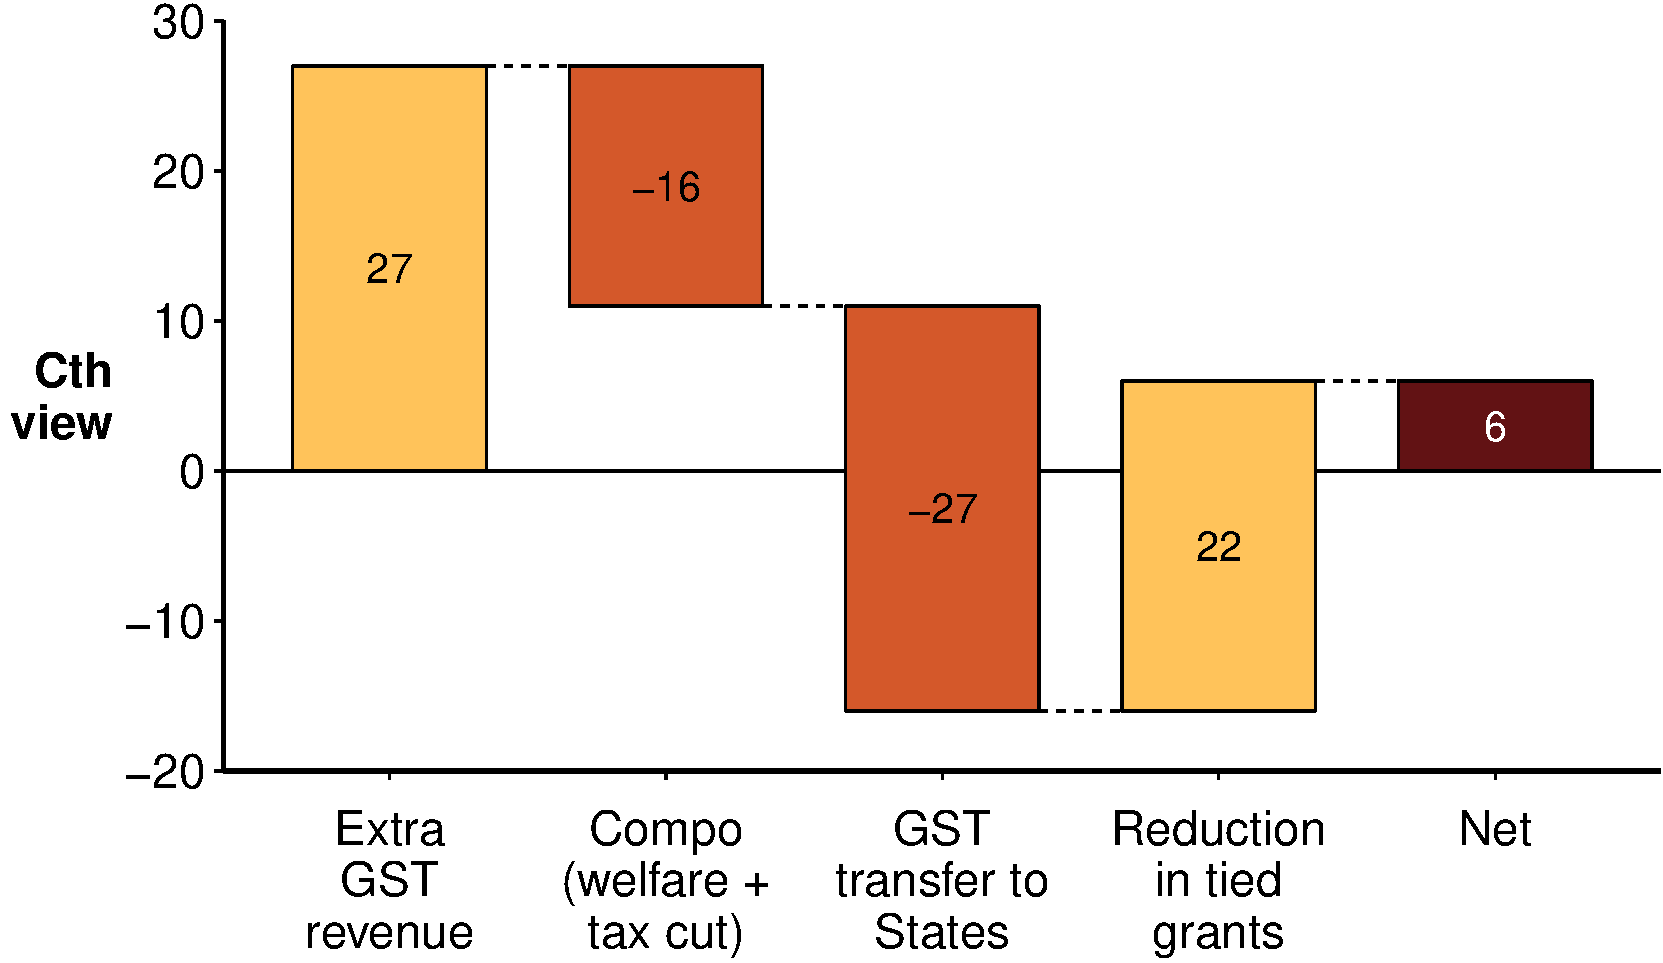
\includegraphics[width=\columnwidth]{atlas/Figure-11-Cth-baptiste.pdf}}
\makebox[\columnwidth][r]{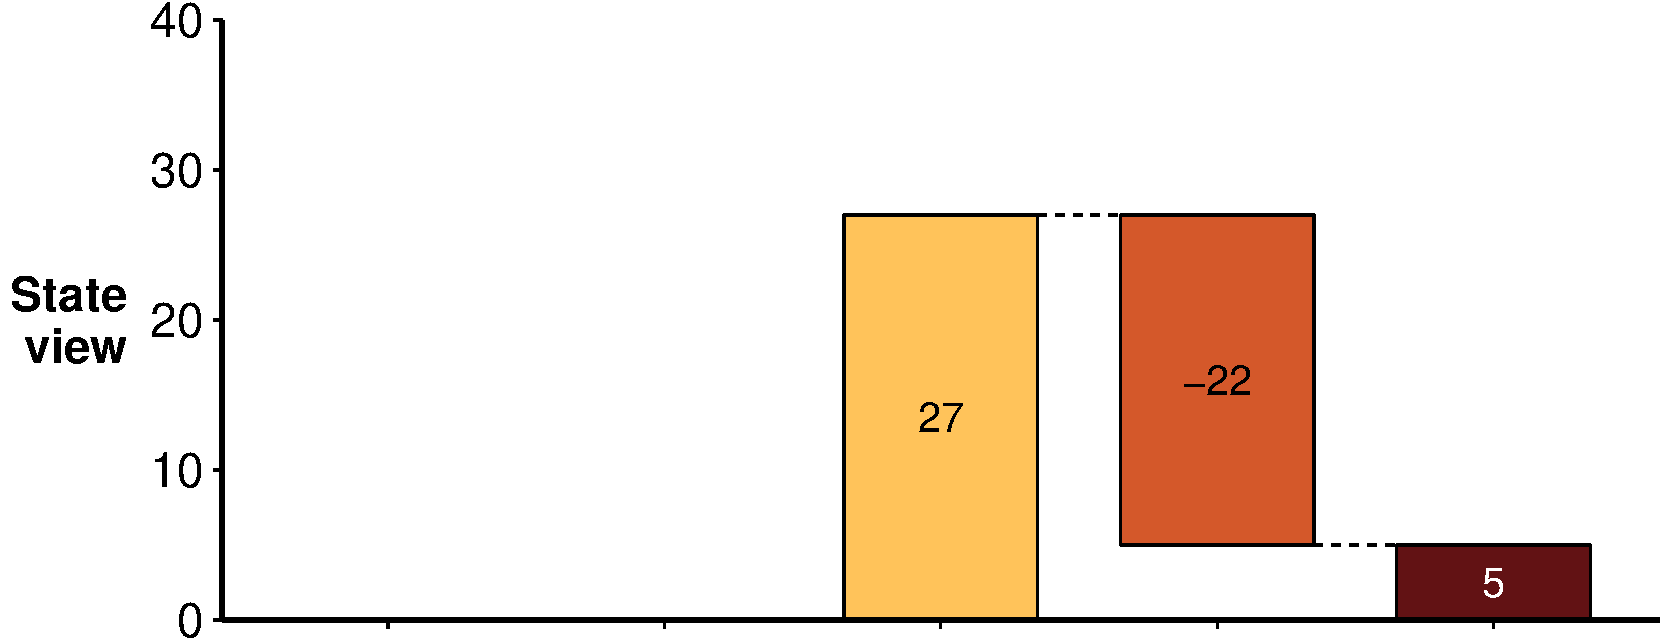
\includegraphics[width=\columnwidth]{atlas/Figure-11-State-baptiste.pdf}}
\source{Grattan analysis}
\end{figure}

Overall, the package we propose provides a sizeable boost to revenues for both the Commonwealth and state governments (\Vref{fig:GST-11}). 

No doubt, both levels of government will quibble about their respective shares. But there is a deal to be done that would support economic growth, make the tax and transfer system more progressive, and give the state and Commonwealth governments more budgetary options. 
